%% abtex2-modelo-trabalho-academico.tex, v-1.9.7 laurocesar
%% Copyright 2012-2018 by abnTeX2 group at http://www.abntex.net.br/ 
%%
%% This work may be distributed and/or modified under the
%% conditions of the LaTeX Project Public License, either version 1.3
%% of this license or (at your option) any later version.
%% The latest version of this license is in
%%   http://www.latex-project.org/lppl.txt
%% and version 1.3 or later is part of all distributions of LaTeX
%% version 2005/12/01 or later.
%%
%% This work has the LPPL maintenance status `maintained'.
%% 
%% The Current Maintainer of this work is the abnTeX2 team, led
%% by Lauro César Araujo. Further information are available on 
%% http://www.abntex.net.br/
%%
%% This work consists of the files abntex2-modelo-trabalho-academico.tex,
%% abntex2-modelo-include-comandos and abntex2-modelo-references.bib
%%
% ------------------------------------------------------------------------
% ------------------------------------------------------------------------
% abnTeX2: Modelo de Trabalho Academico (tese de doutorado, dissertacao de
% mestrado e trabalhos monograficos em geral) em conformidade com 
% ABNT NBR 14724:2011: Informacao e documentacao - Trabalhos academicos -
% Apresentacao
% ------------------------------------------------------------------------
% ------------------------------------------------------------------------
%%
%% Documento ajustado para PCS-EPUSP em 15/mar/2023 por Cintia Borges Margi
% ------------------------------------------------------------------------
%%
\documentclass[
	% -- opções da classe memoir --
	12pt,				% tamanho da fonte
	openright,			% capítulos começam em pág ímpar (insere página vazia caso preciso)
	twoside,			% para impressão em recto e verso. Oposto a oneside
	a4paper,			% tamanho do papel. 
	% -- opções da classe abntex2 --
	%chapter=TITLE,		% títulos de capítulos convertidos em letras maiúsculas
	%section=TITLE,		% títulos de seções convertidos em letras maiúsculas
	%subsection=TITLE,	% títulos de subseções convertidos em letras maiúsculas
	%subsubsection=TITLE,% títulos de subsubseções convertidos em letras maiúsculas
	% -- opções do pacote babel --
	english,			% idioma adicional para hifenização
	%french,				% idioma adicional para hifenização
	%spanish,			% idioma adicional para hifenização
	brazilian				% o último idioma é o principal do documento
	]{abntex2}

% ---
% Pacotes básicos 
% ---
\usepackage{lmodern}			% Usa a fonte Latin Modern			
\usepackage[T1]{fontenc}		% Selecao de codigos de fonte.
\usepackage[utf8]{inputenc}		% Codificacao do documento (conversão automática dos acentos)
\usepackage{indentfirst}		% Indenta o primeiro parágrafo de cada seção.
\usepackage{color}				% Controle das cores
\usepackage{graphicx}			% Inclusão de gráficos
\usepackage{microtype} 			% para melhorias de justificação
\usepackage{silence}
\WarningFilter{babel}{Name 'brazil' is deprecated.}
\WarningFilter{memoir}{\settocpreprocessor is marked deprecated and will be}
% ---
		
% ---
% Pacotes adicionais, usados apenas no âmbito do Modelo Canônico do abnteX2
% ---
\usepackage{lipsum}				% para geração de dummy text
% ---

% ---
% Pacotes de citações
% ---
\usepackage[brazilian,hyperpageref]{backref}	 % Paginas com as citações na bibl
\usepackage[alf]{abntex2cite}	% Citações padrão ABNT

%% CBM: pacote para incluir a ficha catalográfica como pdf
\usepackage[final]{pdfpages}

% --- 
% CONFIGURAÇÕES DE PACOTES
% --- 

% ---
% Configurações do pacote backref
% Usado sem a opção hyperpageref de backref
\renewcommand{\backrefpagesname}{Citado na(s) página(s):~}
% Texto padrão antes do número das páginas
\renewcommand{\backref}{}
% Define os textos da citação
\renewcommand*{\backrefalt}[4]{
	\ifcase #1 %
		Nenhuma citação no texto.%
	\or
		Citado na página #2.%
	\else
		Citado #1 vezes nas páginas #2.%
	\fi}%
% ---

% ---
% Informações de dados para CAPA e FOLHA DE ROSTO
% ---
\titulo{Implementação de Segurança Integrada em Redes LoRaWAN: Detecção de Anomalias via TinyML e Criptografia Leve Ascon.}
\autor{Felpe Luis Korbes, Celso Tadaki Sinoka, João Baréa e Silva}
\local{São Paulo, SP}
\data{2026}
\orientador{Prof. Dr. Victor Takashi Hayashi}
% \coorientador{Alguém?}
\instituicao{%
  Universidade de São Paulo -- USP
  \par
  Escola Politécnica
  \par
  Departamento de Engenharia de Computação e Sistemas Digitais (PCS)}
\tipotrabalho{Monografia de Conclusão de curso (Graduação)}
% O preambulo deve conter o tipo do trabalho, o objetivo, 
% o nome da instituição e a área de concentração 
\preambulo{Trabalho de conclusão de curso apresentado ao Departamento de Engenharia de Computação e Sistemas Digitais da Escola Politécnica da Universidade de São Paulo para obtenção do Título de Engenheiro.}
% ---


% ---
% Configurações de aparência do PDF final

% alterando o aspecto da cor azul
\definecolor{blue}{RGB}{41,5,195}

% informações do PDF
\makeatletter
\hypersetup{
     	%pagebackref=true,
		pdftitle={\@title}, 
		pdfauthor={\@author},
    	pdfsubject={\imprimirpreambulo},
	    pdfcreator={LaTeX with abnTeX2},
		pdfkeywords={abnt}{latex}{abntex}{abntex2}{trabalho acadêmico}, 
		colorlinks=true,       		% false: boxed links; true: colored links
    	linkcolor=blue,          	% color of internal links
    	citecolor=blue,        		% color of links to bibliography
    	filecolor=magenta,      		% color of file links
		urlcolor=blue,
		bookmarksdepth=4
}
\makeatother
% --- 

% ---
% Posiciona figuras e tabelas no topo da página quando adicionadas sozinhas
% em um página em branco. Ver https://github.com/abntex/abntex2/issues/170
\makeatletter
\setlength{\@fptop}{5pt} % Set distance from top of page to first float
\makeatother
% ---

% ---
% Possibilita criação de Quadros e Lista de quadros.
% Ver https://github.com/abntex/abntex2/issues/176
%
\newcommand{\quadroname}{Quadro}
\newcommand{\listofquadrosname}{Lista de quadros}

\newfloat[chapter]{quadro}{loq}{\quadroname}
\newlistof{listofquadros}{loq}{\listofquadrosname}
\newlistentry{quadro}{loq}{0}

% configurações para atender às regras da ABNT
\setfloatadjustment{quadro}{\centering}
\counterwithout{quadro}{chapter}
\renewcommand{\cftquadroname}{\quadroname\space} 
\renewcommand*{\cftquadroaftersnum}{\hfill--\hfill}

\setfloatlocations{quadro}{hbtp} % Ver https://github.com/abntex/abntex2/issues/176
% ---

% --- 
% Espaçamentos entre linhas e parágrafos 
% --- 

% O tamanho do parágrafo é dado por:
\setlength{\parindent}{1.3cm}

% Controle do espaçamento entre um parágrafo e outro:
\setlength{\parskip}{0.2cm}  % tente também \onelineskip

% ---
% compila o indice
% ---
\makeindex
% ---

% ----
% Início do documento
% ----
\begin{document}

% Seleciona o idioma do documento (conforme pacotes do babel)
%\selectlanguage{english}
\selectlanguage{brazilian}
\hypersetup{pageanchor=false}

% Retira espaço extra obsoleto entre as frases.
\frenchspacing
\raggedbottom
\vbadness=10000 

% ----------------------------------------------------------
% ELEMENTOS PRÉ-TEXTUAIS
% ----------------------------------------------------------
% \pretextual

% ---
% Capa
% ---
\imprimircapa
% ---

% ---
% Folha de rosto
% (o * indica que haverá a ficha bibliográfica)
% ---
\imprimirfolhaderosto*
% ---

% ---
% Inserir a ficha bibliografica
% ---

% Isto é um exemplo de Ficha Catalográfica, ou ``Dados internacionais de
% catalogação-na-publicação''. Você pode utilizar este modelo como referência. 
% Porém, provavelmente a biblioteca da sua universidade lhe fornecerá um PDF
% com a ficha catalográfica definitiva após a defesa do trabalho. Quando estiver
% com o documento, salve-o como PDF no diretório do seu projeto e substitua todo
% o conteúdo de implementação deste arquivo pelo comando abaixo:
%
%% TODO: utilizar a ficha catalográfica gerada em https://www.poli.usp.br/bibliotecas/servicos/catalogacao-na-publicacao
\begin{fichacatalografica}
 \hypersetup{pageanchor=false}
 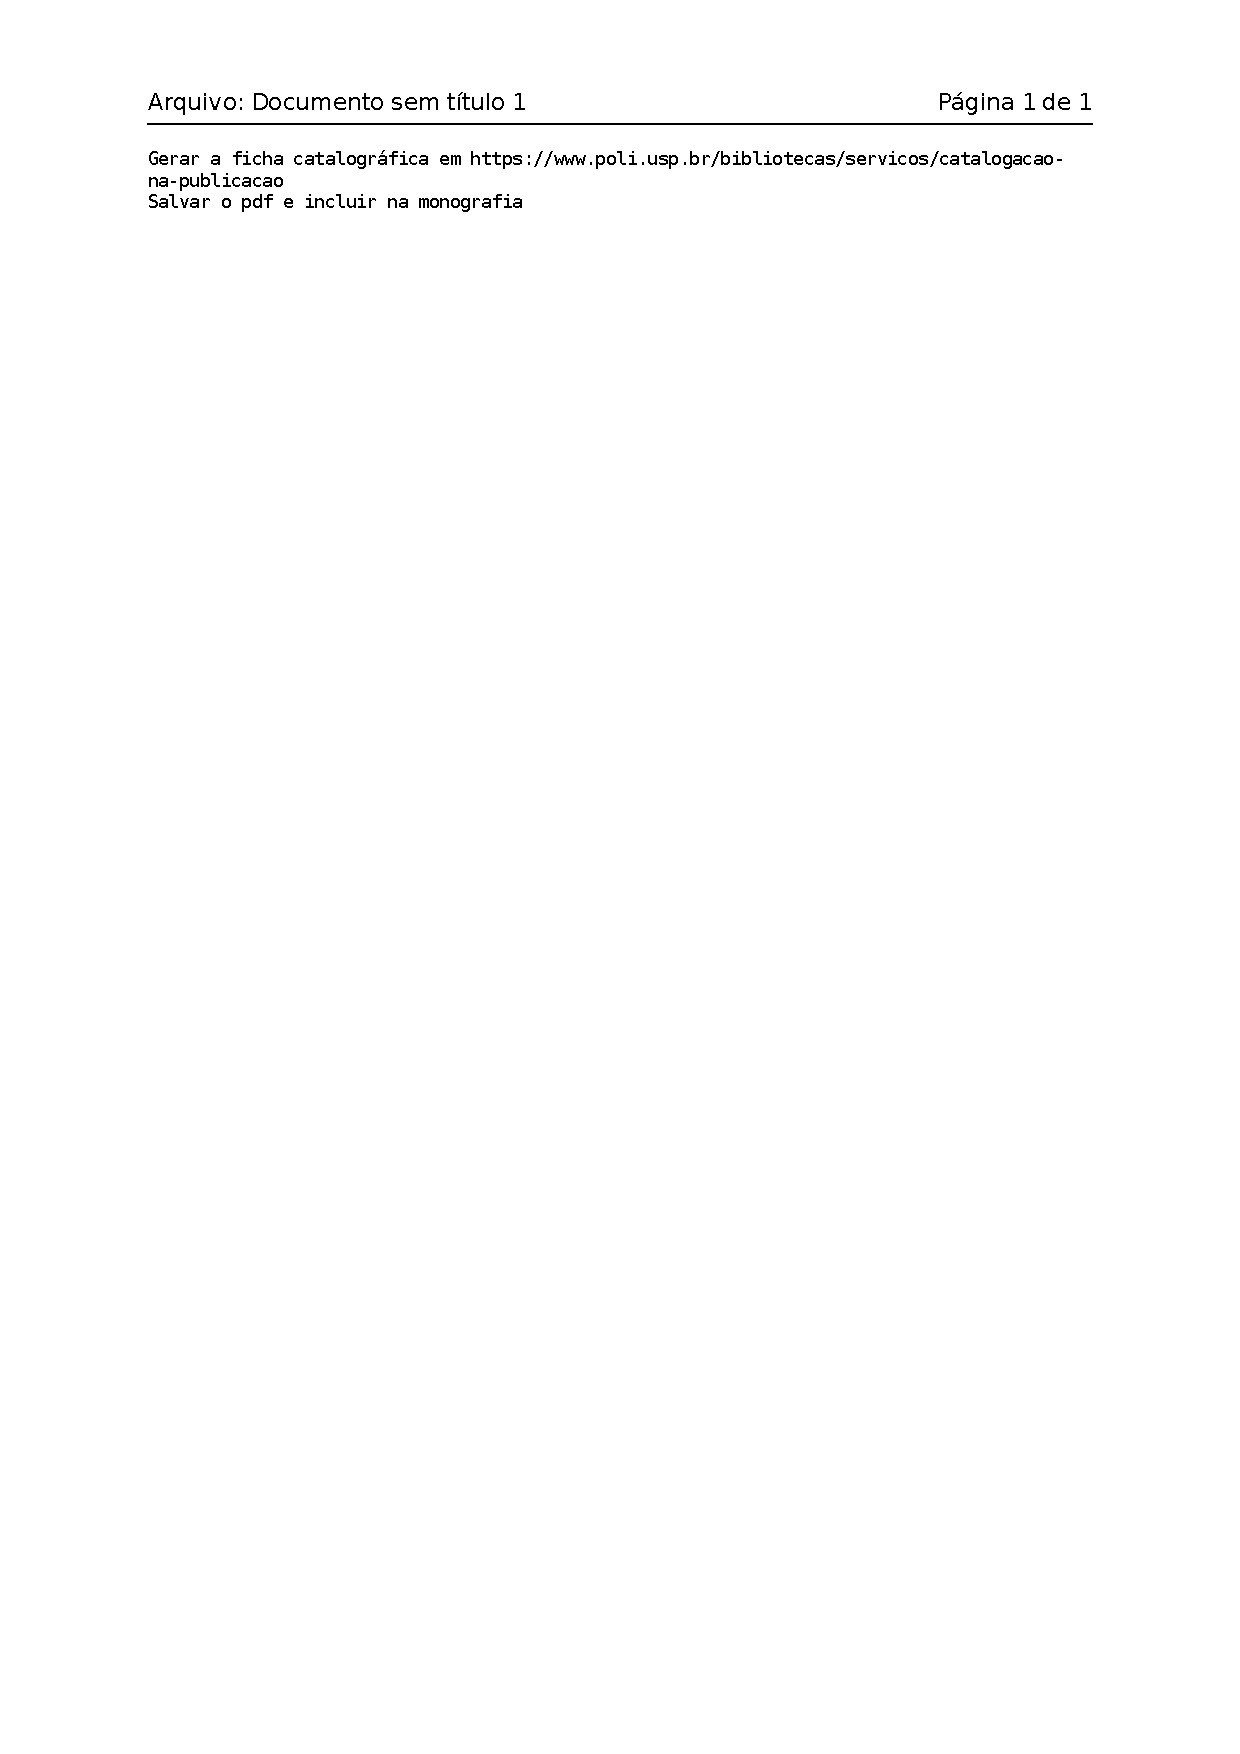
\includepdf{ficha.pdf}
 \hypersetup{pageanchor=true}
\end{fichacatalografica}

% \begin{fichacatalografica}
% 	\sffamily
% 	\vspace*{\fill}					% Posição vertical
% 	\begin{center}					% Minipage Centralizado
% 	\fbox{\begin{minipage}[c][8cm]{13.5cm}		% Largura
% 	\small
% 	\imprimirautor
% 	%Sobrenome, Nome do autor
	
% 	\hspace{0.5cm} \imprimirtitulo  / \imprimirautor. --
% 	\imprimirlocal, \imprimirdata-
	
% 	\hspace{0.5cm} \thelastpage p. : il. (algumas color.) ; 30 cm.\\
	
% 	\hspace{0.5cm} \imprimirorientadorRotulo~\imprimirorientador\\
	
% 	\hspace{0.5cm}
% 	\parbox[t]{\textwidth}{\imprimirtipotrabalho~--~\imprimirinstituicao,
% 	\imprimirdata.}\\
	
% 	\hspace{0.5cm}
% 		1. Palavra-chave1.
% 		2. Palavra-chave2.
% 		3. Palavra-chave3.
% 		I. Orientador.
% 		II. Universidade xxx.
% 		III. Faculdade de xxx.
% 		IV. Título 			
% 	\end{minipage}}
% 	\end{center}
% \end{fichacatalografica}
% ---

% ---
% Inserir errata
% ---
% \begin{errata}
% Elemento opcional da \citeonline[4.2.1.2]{NBR14724:2011}. Exemplo:

% \vspace{\onelineskip}

% FERRIGNO, C. R. A. \textbf{Tratamento de neoplasias ósseas apendiculares com
% reimplantação de enxerto ósseo autólogo autoclavado associado ao plasma
% rico em plaquetas}: estudo crítico na cirurgia de preservação de membro em
% cães. 2011. 128 f. Tese (Livre-Docência) - Faculdade de Medicina Veterinária e
% Zootecnia, Universidade de São Paulo, São Paulo, 2011.

% \begin{table}[htb]
% \center
% \footnotesize
% \begin{tabular}{|p{1.4cm}|p{1cm}|p{3cm}|p{3cm}|}
%   \hline
%    \textbf{Folha} & \textbf{Linha}  & \textbf{Onde se lê}  & \textbf{Leia-se}  \\
%     \hline
%     1 & 10 & auto-conclavo & autoconclavo\\
%    \hline
% \end{tabular}
% \end{table}

% \end{errata}
% ---

% ---
% Inserir folha de aprovação
% ---

% Isto é um exemplo de Folha de aprovação, elemento obrigatório da NBR
% 14724/2011 (seção 4.2.1.3). Você pode utilizar este modelo até a aprovação
% do trabalho. Após isso, substitua todo o conteúdo deste arquivo por uma
% imagem da página assinada pela banca com o comando abaixo:
%
% \begin{folhadeaprovacao}
% \includepdf{folhadeaprovacao_final.pdf}
% \end{folhadeaprovacao}
%
% \begin{folhadeaprovacao}

%   \begin{center}
%     {\ABNTEXchapterfont\large\imprimirautor}

%     \vspace*{\fill}\vspace*{\fill}
%     \begin{center}
%       \ABNTEXchapterfont\bfseries\Large\imprimirtitulo
%     \end{center}
%     \vspace*{\fill}
    
%     \hspace{.45\textwidth}
%     \begin{minipage}{.5\textwidth}
%         \imprimirpreambulo
%     \end{minipage}%
%     \vspace*{\fill}
%    \end{center}
        
%    Trabalho aprovado. \imprimirlocal, 24 de novembro de 2012:

%    \assinatura{\textbf{\imprimirorientador} \\ Orientador} 
%    \assinatura{\textbf{Professor} \\ Convidado 1}
%    \assinatura{\textbf{Professor} \\ Convidado 2}
%    %\assinatura{\textbf{Professor} \\ Convidado 3}
%    %\assinatura{\textbf{Professor} \\ Convidado 4}
      
%    \begin{center}
%     \vspace*{0.5cm}
%     {\large\imprimirlocal}
%     \par
%     {\large\imprimirdata}
%     \vspace*{1cm}
%   \end{center}
  
% \end{folhadeaprovacao}
% ---

% ---
% Dedicatória
% ---
\begin{dedicatoria}
   \vspace*{\fill}
   \centering
   \noindent
   \textit{Este trabalho é dedicado às crianças adultas que,\\
   quando pequenas, sonharam em se tornar cientistas.} \vspace*{\fill}
\end{dedicatoria}
% ---

% ---
% Agradecimentos
% ---
%\begin{agradecimentos}
%Os agradecimentos principais são direcionados ...

%\end{agradecimentos}
% ---

% ---
% Epígrafe
% ---
% \begin{epigrafe}
%     \vspace*{\fill}
% 	\begin{flushright}
% 		\textit{...}
% 	\end{flushright}
% \end{epigrafe}
% ---

% ---
% RESUMOS
% ---

% resumo em português
% O resumo deve ressaltar o  objetivo, o método, os resultados e as conclusões do documento. 
% Deve ser escrito em parágrafo única, e tipicamente é menor do que uma página.(\ldots) 
% As palavras-chave devem figurar logo abaixo do resumo, antecedidas da expressão Palavras-chave:, 
% separadas entre si por ponto e finalizadas também por ponto.
\setlength{\absparsep}{18pt} % ajusta o espaçamento dos parágrafos do resumo
\begin{resumo}
A segurança da informação no protocolo \textit{Long Range Wide Area Network} LoRaWAN é um desafio crítico para aplicações de Internet das Coisas (IoT), devido à vulnerabilidade a ataques, como \textit{jamming}, \textit{spoofing}, DoS e \textit{Man-in-the-middle}, combinada às rigorosas restrições energéticas e computacionais dos dispositivos de borda. Diante desse cenário, o presente trabalho tem como objetivo desenvolver e avaliar uma arquitetura de segurança integrada para dispositivos embarcados. A metodologia proposta baseia-se na implementação do algoritmo de criptografia leve Ascon, visando garantir a confidencialidade e integridade dos dados, operando em conjunto com um modelo de aprendizado de máquina focado na detecção de anomalias e intrusões no tráfego da rede. O protótipo será construído utilizando microcontroladores com restrição de recursos. Espera-se que a integração do padrão Ascon com a detecção com o aprendizado de máquina mitigue vetores de ataque comuns em redes LoRaWAN sem inviabilizar a operação sustentável dos dispositivos, resultando em uma solução robusta, autônoma e aplicável a ambientes de automação industrial e cidades inteligentes.

 \textbf{Palavras-chave}: LoRaWAN; IoT; Detecção de Anomalias; Criptografia Leve.
\end{resumo}

% resumo em inglês
\begin{resumo}[Abstract]
 \begin{otherlanguage*}{english}
   Information security in the LoRaWAN protocol is a critical challenge for Internet of Things (IoT) applications, due to vulnerability to attacks such as \textit{jamming}, \textit{spoofing}, DoS, and \textit{Man-in-the-middle}, combined with the strict energy and computational constraints of edge devices. In this context, the present work aims to develop and evaluate an integrated security architecture for embedded devices. The proposed methodology is based on the implementation of the lightweight cryptographic algorithm Ascon to ensure data confidentiality and integrity, operating alongside a machine learning model focused on the detection of anomalies and intrusions in network traffic. The prototype will be built using resource-constrained microcontrollers. It is expected that integrating the Ascon standard with anomaly detection through machine learning will mitigate common attack vectors in LoRaWAN networks without compromising the sustainable operation of the devices, resulting in a robust, autonomous solution applicable to industrial automation and smart city environments.

   \vspace{\onelineskip}
 
   \noindent 
   \textbf{Keywords}: LoRaWAN; IoT; Anomaly Detection; Lightweight Cryptography.
 \end{otherlanguage*}
\end{resumo}

% % resumo em francês 
% \begin{resumo}[Résumé]
%  \begin{otherlanguage*}{french}
%     Il s'agit d'un résumé en français.
 
%    \textbf{Mots-clés}: latex. abntex. publication de textes.
%  \end{otherlanguage*}
% \end{resumo}

% % resumo em espanhol
% \begin{resumo}[Resumen]
%  \begin{otherlanguage*}{spanish}
%    Este es el resumen en español.
  
%    \textbf{Palabras clave}: latex. abntex. publicación de textos.
%  \end{otherlanguage*}
% \end{resumo}
% ---

% ---
% inserir lista de ilustrações
% ---
\pdfbookmark[0]{\listfigurename}{lof}
\listoffigures*
\cleardoublepage
% ---

% ---
% inserir lista de quadros
% ---
%\pdfbookmark[0]{\listofquadrosname}{loq}
%\listofquadros*
%\cleardoublepage
% ---

% ---
% inserir lista de tabelas
% ---
\pdfbookmark[0]{\listtablename}{lot}
\listoftables*
\cleardoublepage
% ---

% ---
% inserir lista de abreviaturas e siglas
% ---
\begin{siglas}
  \item[ABNT] Associação Brasileira de Normas Técnicas
  \item[ABP] Activation by Personalization
  \item[ADR] Adaptive Data Rate
  \item[AEAD] Authenticated Encryption with Associated Data
  \item[AES] Advanced Encryption Standard
  \item[API] Application Programming Interface
  \item[ARIMA] AutoRegressive Integrated Moving Average
  \item[DDoS] Distributed Denial of Service
  \item[DES] Data Encryption Standard
  \item[DoS] Denial of Service
  \item[DRBG] Deterministic Random Bit Generator
  \item[ESP32] Espressif 32
  \item[HTTP] Hypertext Transfer Protocol
  \item[IoT] Internet of Things
  \item[KAT] Known Answer Tests
  \item[LoRa] Long Range
  \item[LoRaWAN] Long Range Wide Area Network
  \item[LPWAN] Low-Power Wide-Area Network
  \item[LSTM] Long Short-Term Memory
  \item[MAC] Medium Access Control
  \item[MAE] Mean Absolute Error
  \item[ML] Machine Learning
  \item[NIST] National Institute of Standards and Technology
  \item[OTAA] Over-the-Air Activation
  \item[RAM] Random Access Memory
  \item[RBG] Random Bit Generator
  \item[RF] Rádio Frequência
  \item[RMSE] Root Mean Squared Error
  \item[RNN] Recurrent Neural Network
  \item[RSSI] Received Signal Strength Indicator
  \item[SNR] Signal-to-Noise Ratio
  \item[TinyML] Tiny Machine Learning
  \item[TRNG] True Random Number Generator
\end{siglas}
% ---

% ---
% inserir lista de símbolos
% ---
\begin{simbolos}
  \item[$K$] Chave criptográfica derivada
  \item[$U$] Sequência de bits do gerador aleatório aprovado
  \item[$V$] Sequência de bits independente usada na derivação
  \item[$\oplus$] Operação XOR (ou-exclusivo)
  \item[$\lambda$] Tamanho da \textit{tag} de autenticação (em bits)
  \item[$\leq$] Relação menor ou igual
\end{simbolos}
% ---

% ---
% inserir o sumario
% ---
\pdfbookmark[0]{\contentsname}{toc}
\tableofcontents*
\cleardoublepage
% ---


% ----------------------------------------------------------
% ELEMENTOS TEXTUAIS
% ----------------------------------------------------------
\hypersetup{pageanchor=true}
\textual

% Capítulo 1. Introdução
\chapter{Introdução} \label{cap:introducao}

A Internet das Coisas (IoT) é composta por dispositivos embarcados que desempenham funções específicas, atuando como sensores e controladores para uma variedade de aplicações tecnológicas produzidas hoje em dia, desde os aparelhos mais simples do cotidiano até processos industriais complexos. Com a evolução do hardware, os dispositivos IoT tornaram-se menores, mais rápidos, mais eficientes e com menor custo, o que levou a uma explosão do seu uso \cite{alfuqaha2015iot}.

Contudo, um dos principais entraves para essa tecnologia decorre das limitações energéticas e computacionais desses dispositivos \cite{nistir8114}. Apesar da evolução vista nas últimas décadas, a IoT ainda enfrenta gargalos em processos que demandam alto poder computacional, devido à grande carga de processamento e ao elevado custo energético.

Diante desse cenário, surgem questões de segurança que podem ser exploradas para invadir e comprometer o funcionamento da rede. Para resolver a questão da transmissão segura e eficiente, padrões como o ASCON, pela necessidade de se padronizar e produzir um conjunto de métodos criptográficos que sejam leves para uso em dispositivos com baixo consumo energético \cite{nist800232}. Em paralelo, para viabilizar a comunicação de longa distância com baixa energia, utiliza-se amplamente o protocolo LoRaWAN, que possui aplicações fundamentais em diversas áreas, desde a infraestrutura de cidades inteligentes e controle de tráfego até o monitoramento de desastres, agricultura de precisão e automação industrial com foco em manutenção preditiva. O grande problema enfrentado por esse protocolo, no entanto, é a 
segurança da informação frente a ataques como jamming, replay attacks, 
spoofing e denial of service \cite{hessel2023lorawan}. A vulnerabilidade a ataques podem causar disrupções críticas e prejuízos severos, tornando indispensável a aplicação de métodos robustos de prevenção. 

%%%%%%%%%%%%%%%%%%%%%%%%%%%%%%%%%%%%%%%%%%%%%%%%%%%%
%%%%%%%%%%%%%%%%%%%%%%%%%%%%%%%%%%%%%%%%%%%%%%%%%%%%

\section{Motivação}
A necessidade de operar com baixo consumo energético eleva bastante a complexidade do uso de dispositivos IoT, uma vez que tentativas de mitigar esse problema podem resultar em simplificações que geram problemas de segurança \cite{nistir8114} \cite{hessel2023lorawan}. Diante disso, torna-se pertinente compreender a natureza desses ataques e suas formas de mitigação, além de estudar a eficiência e a eficácia de modelos de Machine Learning na detecção de intrusões e anomalias.

Um desses problemas é a vulnerabilidade a ataques diretos, como ataques de negação de serviço (DDoS) ou Jamming, que podem esgotar a bateria do dispositivo ou impedir que a coleta de dados seja feita de maneira adequada \cite{hessel2023lorawan}. Outro grande desafio está na comunicação: é preciso garantir que a informação transmitida entre os dispositivos não possa ser interceptada nem modificada, assegurando a integridade, confidencialidade e autenticidade dos dados. Como os algoritmos de segurança comumente utilizados exigem um grande poder computacional, torna-se necessário buscar maneiras mais eficientes de proteger os dados durante a transmissão.


O uso de \textit{Machine Learning} neste trabalho decorre da necessidade de 
detectar anomalias em redes LoRaWAN a partir de padrões temporais e 
comportamentais dos dados. Em contextos reais de IoT, abordagens baseadas 
apenas em regras fixas ou limiares estáticos tendem a ser limitadas. O 
comportamento normal pode variar conforme o contexto operacional (dispositivo, 
gateway, ambiente) e evoluir ao longo do tempo, tornando limiares fixos 
(ex: ``se RSSI < -120 dBm, alertar'') inadequados. Além disso, métodos 
tradicionais apresentam dificuldade em capturar estruturas complexas em dados 
sequenciais, tais como degradação gradual de equipamento ou padrões não 
lineares de transmissão. Por outro lado, abordagens baseadas em aprendizado 
conseguem modelar relações temporais, identificar desvios sutis e adaptar-se 
dinamicamente à evolução do comportamento normal, mostrando-se mais adequadas 
para este contexto \cite{chalapathy2019}.

Por isso, a modelagem é realizada com base no comportamento esperado do dispositivo em suas circunstâncias normais de operação, buscando aprender padrões legítimos de funcionamento a partir dos dados observados. Nessa abordagem, desvios suficientemente relevantes em relação ao comportamento previamente aprendido são tratados como indícios de anomalia. Trata-se, portanto, de uma abordagem adaptativa, pois o modelo se ajusta ao perfil comportamental de cada nó monitorado. \cite{hayashi2022handsfree}.


Assim, neste trabalho, \textit{Machine Learning} é tratado como um dos núcleos centrais da investigação. Seu papel não é apenas classificar dados, mas aprender perfis de operação, comparar abordagens de detecção e oferecer uma base experimental para uma etapa posterior de avaliação em borda. Essa decisão amplia o escopo da análise, permitindo estudar simultaneamente eficácia de detecção, robustez metodológica e viabilidade de implantação em borda.

O padrão Ascon, por sua vez, foi selecionado como a primeira escolha como novo padrão da competição de criptografia leve do NIST \citeonline{nist_lwc_finalists} assim como a primeira escolha de criptografia leve da competição CAESAR \cite{caesar_submissions}. A relevância desse padrão se torna clara quando analisado seu baixo custo energético, rapidez, e confiabilidade, garantindo segurança para dados AEAD e ataques de canal colateral \cite{ascon_official}.

%%%%%%%%%%%%%%%%%%%%%%%%%%%%%%%%%%%%%%%%%%%%%%%%%%%%
%%%%%%%%%%%%%%%%%%%%%%%%%%%%%%%%%%%%%%%%%%%%%%%%%%%%

\section{Objetivos}
O objetivo geral deste trabalho é implementar e avaliar um sistema de comunicação baseado no protocolo LoRaWAN, integrando a aplicação de modelos de \textit{Machine Learning} e o padrão de criptografia leve Ascon. A finalidade central é analisar o nível de segurança e a resiliência que a combinação dessas duas tecnologias pode oferecer ao ecossistema de Internet das Coisas (IoT).

Para o alcance do objetivo geral, foram definidos os seguintes objetivos específicos:

\begin{itemize}
    \item Treinar e testar modelos de \textit{Machine Learning}, utilizando os \textit{datasets} selecionados, para atuar na identificação e mitigação de ameaças ativas, tais como \textit{jamming}, \textit{spoofing} e ataques de Negação de Serviço (DoS).
    \item Implementar os algoritmos da família Ascon no nó sensor para estabelecer uma infraestrutura que garanta a privacidade, a autenticidade e a integridade dos dados transmitidos, com baixo custo computacional.
    \item Desenvolver o protótipo do sistema integrando as camadas de comunicação (LoRaWAN), de detecção e criptografia.
    \item Analisar o nível de segurança global oferecido pelo conjunto, validando a eficácia da solução proposta frente às restrições do hardware - em termos de consumo energético.
\end{itemize}

%%%%%%%%%%%%%%%%%%%%%%%%%%%%%%%%%%%%%%%%%%%%%%%%%%%%
%%%%%%%%%%%%%%%%%%%%%%%%%%%%%%%%%%%%%%%%%%%%%%%%%%%%

\section{Justificativa}
A relevância deste trabalho evidencia-se pelo papel central e pela rápida expansão dos dispositivos de Internet das Coisas (IoT) no cotidiano, com projeções indicando dezenas de bilhões de equipamentos conectados nos próximos anos \cite{pandey2025}. Propor uma metodologia que integra tecnologias e conceitos críticos como o protocolo de comunicação LoRaWAN, modelos de \textit{Machine Learning} e segurança criptográfica, e verificar a sua eficácia em cenários práticos, demonstra como a união dessas ferramentas pode alavancar a resiliência de sistemas reais, tornando-os cada vez mais robustos contra ameaças.

%%%%%%%%%%%%%%%%%%%%%%%%%%%%%%%%%%%%%%%%%%%%%%%%%%%%
%%%%%%%%%%%%%%%%%%%%%%%%%%%%%%%%%%%%%%%%%%%%%%%%%%%%

\section{Organização do Trabalho}
Para facilitar a leitura e a compreensão da pesquisa, este documento está estruturado da seguinte forma:

O Capítulo \ref{cap:conceitos} apresenta os aspectos conceituais que fundamentam o projeto. Nele, são abordados o funcionamento do protocolo LoRaWAN e o paradigma da criptografia leve (\textit{Lightweight Cryptography}), detalhando o processo de padronização do NIST que elegeu a família Ascon, além de uma comparação com outras famílias de algoritmos. O capítulo também explora a base teórica de \textit{Machine Learning} voltada para a detecção de anomalias.

O Capítulo \ref{cap:metodo} descreve o método do trabalho. Primeiramente, apresenta-se a 
abordagem de elicitação de requisitos adotada, incluindo análise de 
literatura, identificação de restrições de hardware e validação de 
viabilidade técnica. Em seguida, são detalhados os datasets analisados e 
selecionados para o modelo de Machine Learning, os procedimentos de 
treinamento e avaliação, bem como a justificativa para a adoção da 
biblioteca ascon-suite na implementação do padrão Ascon. O capítulo abrange 
ainda as etapas de configuração do ambiente, implementação e métodos de teste.

O Capítulo \ref{cap:especificacao} trata da especificação de requisitos do sistema, definindo as restrições computacionais, de memória e de consumo energético que o protótipo deve respeitar para operar na borda da rede.

O Capítulo \ref{cap:desenvolvimento} é dedicado ao projeto e desenvolvimento. Nesta etapa, são descritas as tecnologias e ferramentas práticas utilizadas, a arquitetura montada, os testes realizados e a discussão dos resultados obtidos.

Por fim, o Capítulo \ref{cap:consideracoes} apresenta as considerações finais, sumarizando as conclusões extraídas da pesquisa e apontando direcionamentos para futuras implementações e melhorias que podem surgir a partir deste trabalho.

% Capítulo 2. Aspectos Conceituais
\chapter{Aspectos Conceituais} \label{cap:conceitos}


A proteção efetiva de um sistema não é alcançada por uma única técnica, 
mas pela combinação de estratégias em múltiplas camadas. Conforme o 
\textit{NIST Cybersecurity Framework} \cite{nist_csf_2024}, a segurança 
robusta exige tanto \textbf{prevenção} (impedindo que ataques ocorram) 
quanto \textbf{detecção} (identificando atividades suspeitas). Este 
capítulo apresenta os conceitos que fundamentam este trabalho dentro 
desse paradigma: protocolos de comunicação para IoT, criptografia leve 
como mecanismo preventivo, e Machine Learning como mecanismo de detecção 
comportamental.


\section{Redes IoT e o Protocolo LoRaWAN}

As redes de Internet das Coisas (IoT) utilizam amplamente o protocolo LoRaWAN em cenários que exigem baixo consumo de energia e ampla cobertura. Embora o LoRaWAN apresente certa maturidade e conte com mecanismos de proteção continuamente aprimorados, ataques e problemas de segurança ainda afetam sua resiliência. Consequentemente, permanece necessária a evolução contínua de técnicas de prevenção e mitigação dessas ameaças \cite{hessel2023lorawan}.

%%%%%%%%%%%%%%%%%%%%%%%%%%%%%%%%%%%%%%%%%%%%%%%%%%%%

\subsection{LoRa e LoRaWAN: fundamentos e evolução do protocolo}

O LoRaWAN se destaca como uma tecnologia voltada a redes LPWAN (\textit{Low-Power Wide-Area Network}), sendo utilizado em aplicações como monitoramento remoto, agricultura inteligente e sistemas distribuídos com dispositivos embarcados. Sua proposta é permitir a comunicação entre dispositivos com baixo consumo energético, ampla cobertura e custo operacional reduzido.

É importante distinguir os termos \textit{LoRa} e \textit{LoRaWAN}, que frequentemente são tratados como sinônimos, embora representem camadas diferentes da tecnologia. O LoRa corresponde à camada física da comunicação, isto é, à técnica de modulação empregada no enlace sem fio. Já o LoRaWAN define o protocolo de comunicação acima dessa camada, estabelecendo regras para organização da rede, troca de mensagens e controle da comunicação. Em outras palavras, o LoRa fornece o meio de transmissão por rádio, enquanto o LoRaWAN define o funcionamento da rede sobre esse meio.

De forma geral, o LoRaWAN foi projetado para redes compostas por dispositivos com recursos limitados, muitas vezes alimentados por bateria e instalados em locais de difícil manutenção. Por isso, o protocolo prioriza simplicidade operacional, baixo consumo e comunicação eficiente, ainda que com taxas de transmissão menores do que tecnologias voltadas a maior vazão de dados. Essa característica o torna adequado para cenários em que pequenas quantidades de informação precisam ser transmitidas periodicamente, sem necessidade de comunicação contínua.

A evolução do LoRaWAN também é um aspecto importante. Desde sua primeira publicação, em 2015, o protocolo passou por revisões que resultaram em dois ramos principais: a família 1.0.x e a versão 1.1. As versões da família 1.0.x mantiveram interoperabilidade entre si e trouxeram principalmente correções, esclarecimentos e ajustes incrementais. Já a versão 1.1 introduziu mudanças mais relevantes, especialmente na organização de funções da rede e nos mecanismos de segurança, tornando mais clara a separação entre responsabilidades de rede e de aplicação.

\begin{figure}[htb]
  \caption{\label{lorawan_version_history}Histórico de versionamento da especificação da LoRaWAN}
  \begin{center}
      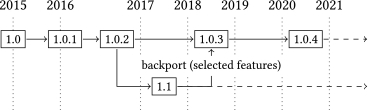
\includegraphics[scale=0.8]{figuras/lorawan_version_history.png}
  \end{center}
  \legend{Fonte: \cite{hessel2023lorawan}}
\end{figure}

Mesmo com a introdução de melhorias nas versões mais recentes, a adoção de novas revisões do protocolo não ocorre de forma imediata em sistemas reais. Em aplicações IoT, sensores podem permanecer em operação por muitos anos, frequentemente sem atualização de firmware. Como consequência, versões anteriores do LoRaWAN continuam relevantes na prática, e essa coexistência entre gerações do protocolo precisa ser considerada em qualquer análise técnica ou experimental.

Assim, compreender a distinção entre LoRa e LoRaWAN, bem como a evolução do protocolo ao longo de suas versões, é essencial para analisar corretamente seu funcionamento em sistemas embarcados conectados. A partir dessa base, as próximas subseções detalham a arquitetura da rede, o processo de ativação dos dispositivos, a transferência de dados, os mecanismos de gerenciamento da comunicação e a relação dessas tecnologias com a arquitetura proposta neste trabalho.

%%%%%%%%%%%%%%%%%%%%%%%%%%%%%%%%%%%%%%%%%%%%%%%%%%%%

\subsection{Arquitetura da Rede}

A arquitetura do LoRaWAN é composta por diferentes entidades, cada uma com uma função específica no funcionamento da rede. De forma geral, os dispositivos finais, chamados de \textit{End Devices}, são responsáveis por coletar e transmitir dados. Esses dispositivos se comunicam por rádio com um ou mais \textit{Gateways}, que atuam como pontes entre a rede LoRa e a infraestrutura conectada por IP. Os gateways, por sua vez, apenas recebem os quadros transmitidos pelos dispositivos e os encaminham para os servidores da rede, sem realizar processamento completo do protocolo. \cite{hessel2023lorawan}

Essa organização forma uma topologia conhecida como \textit{star-of-stars}. Nela, os dispositivos finais não se comunicam diretamente entre si, e também não estabelecem vínculo fixo com um único gateway. Em vez disso, uma mesma transmissão pode ser recebida por vários gateways que estejam dentro de alcance. Essa característica aumenta a cobertura da rede e oferece maior robustez na recepção das mensagens, especialmente em cenários distribuídos e com mobilidade.

\begin{figure}[htb]
  \caption{\label{lorawan_architeture}Arquitetura de rede LoRaWAN}
  \begin{center}
      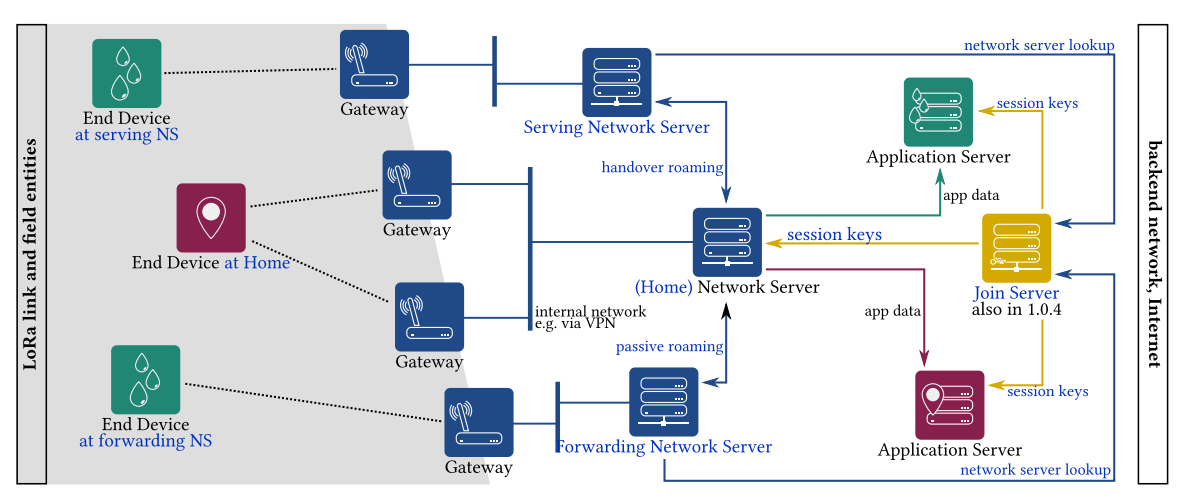
\includegraphics[scale=0.4]{figuras/architeture_LoRaWan.png}
  \end{center}
  \legend{Fonte: \cite{hessel2023lorawan}}
\end{figure}

Após o encaminhamento feito pelos gateways, as mensagens chegam ao \textit{Network Server}. Esse servidor exerce papel central na rede, pois é responsável por processar as mensagens recebidas, eliminar duplicidades causadas pela recepção do mesmo quadro por múltiplos gateways, validar a integridade das mensagens e executar as funções de gerenciamento da camada MAC. Em outras palavras, é o \textit{Network Server} que coordena o funcionamento lógico da rede LoRaWAN.

Os dados de aplicação seguem então para o \textit{Application Server}, que é o componente responsável por tratar a informação útil transportada pelo dispositivo final. É nesse servidor que os dados recebidos podem ser decifrados, interpretados e encaminhados para a aplicação de interesse, como um sistema de monitoramento, um banco de dados ou uma plataforma de análise. Essa separação entre funções de rede e funções de aplicação é importante porque organiza melhor as responsabilidades do sistema e reduz o acoplamento entre comunicação e processamento da informação.

Na evolução do protocolo, especialmente a partir do LoRaWAN 1.1, o \textit{Join Server} passa a ter um papel mais explícito na arquitetura. Esse componente participa do processo de ativação dos dispositivos e da derivação de chaves de sessão, contribuindo para uma separação mais clara entre gerenciamento de rede e segurança da aplicação. Com isso, a arquitetura do LoRaWAN se torna mais organizada do ponto de vista funcional e mais adequada a cenários em que diferentes operadores ou domínios de serviço precisam cooperar.

Assim, a arquitetura do LoRaWAN pode ser entendida como uma organização em camadas funcionais: o dispositivo final coleta e transmite os dados, o gateway encaminha os quadros recebidos, o \textit{Network Server} gerencia a comunicação da rede, e o \textit{Application Server} entrega os dados à aplicação. Nas versões mais recentes, o \textit{Join Server} complementa essa estrutura ao apoiar o processo de ativação e gerenciamento de chaves. Essa divisão de papéis é fundamental para compreender como o protocolo opera e como seus componentes podem ser relacionados à arquitetura proposta neste trabalho.

%%%%%%%%%%%%%%%%%%%%%%%%%%%%%%%%%%%%%%%%%%%%%%%%%%%%

\subsection{Ativação do Dispositivo}

Antes de transmitir dados de aplicação, um dispositivo LoRaWAN precisa ser ativado na rede. Esse processo define como o dispositivo passa a ser reconhecido pelo sistema e como obtém o contexto necessário para a comunicação, incluindo identificadores, parâmetros de sessão e chaves utilizadas ao longo da operação. De forma geral, o LoRaWAN admite dois modos principais de ativação: \textit{Activation By Personalization} (ABP) e \textit{Over-The-Air Activation} (OTAA). \cite{hessel2023lorawan}

No modo ABP, o dispositivo já é configurado previamente com os parâmetros de sessão necessários para operar. Assim, ele pode iniciar a transmissão diretamente, sem realizar um procedimento de ingresso na rede a cada inicialização. Essa abordagem é mais simples do ponto de vista de implementação, mas oferece menor flexibilidade operacional, já que os parâmetros de comunicação ficam previamente fixados no dispositivo.

No modo OTAA, por outro lado, o dispositivo realiza um procedimento de ingresso na rede antes de iniciar sua operação normal. Nesse processo, o nó envia uma solicitação de ativação e, a partir da resposta da infraestrutura da rede, passa a operar com parâmetros e chaves de sessão derivados especificamente para aquela conexão. Em comparação com o ABP, essa abordagem é mais flexível e mais adequada a cenários reais, pois facilita renovação de chaves, adaptação do contexto de comunicação e suporte a funcionalidades mais avançadas do protocolo.

De forma simplificada, a ativação por OTAA envolve a troca de mensagens de ingresso e a geração de chaves de sessão a partir de credenciais previamente associadas ao dispositivo. Esse mecanismo permite que a rede estabeleça uma nova sessão de comunicação de forma controlada, em vez de depender sempre de parâmetros estáticos. Por esse motivo, o OTAA tende a ser considerado a alternativa mais robusta para implantações práticas, especialmente quando se deseja maior controle do ciclo de vida dos dispositivos e melhor suporte a segurança.

\begin{figure}[htb]
  \caption{\label{lorawan_join_process} (a) OTAA processo de entrada LoRaWAN 1.0.x. (b) OTAA processo de entrada LoRaWAN 1.1}
  \begin{center}
      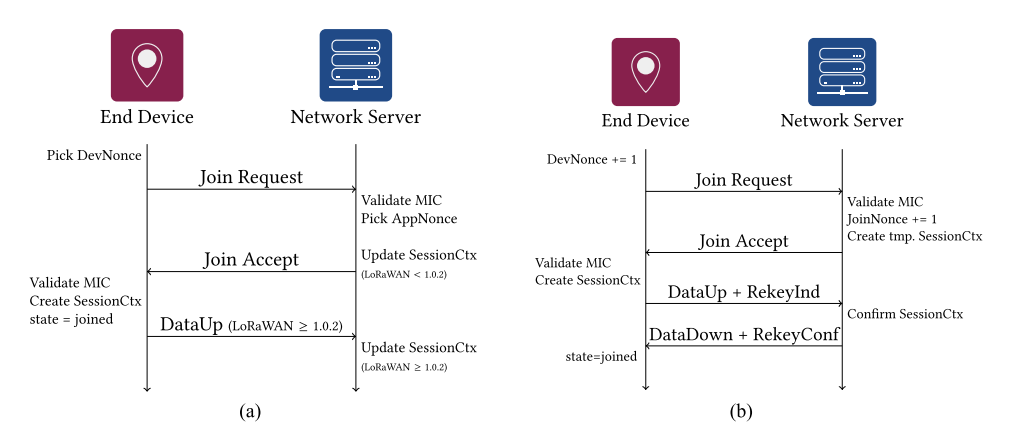
\includegraphics[scale=0.4]{figuras/otaa_join_process.png}
  \end{center}
  \legend{Fonte: \cite{hessel2023lorawan}}
\end{figure}

A evolução do protocolo também impacta esse processo. Nas versões da família 1.0.x, a ativação já podia ocorrer por ABP ou OTAA, mas a versão 1.1 introduziu uma separação mais clara entre funções de rede e aplicação, além de mudanças no tratamento das chaves e no papel do \textit{Join Server}. Com isso, o processo de ativação passou a ser mais estruturado e alinhado com uma arquitetura de segurança mais organizada.

Assim, a ativação do dispositivo representa uma etapa fundamental no funcionamento do LoRaWAN, pois estabelece as condições iniciais para que a comunicação ocorra de forma válida dentro da rede. Enquanto o ABP oferece uma alternativa mais simples, o OTAA apresenta maior flexibilidade e melhor aderência a cenários práticos e escaláveis. A partir dessa etapa, o dispositivo pode iniciar a troca de dados com a infraestrutura da rede, conforme discutido na próxima subseção.

%%%%%%%%%%%%%%%%%%%%%%%%%%%%%%%%%%%%%%%%%%%%%%%%%%%%

\subsection{Transferência de Dados}

Após a ativação do dispositivo, a comunicação de dados pode ocorrer entre o dispositivo final e a infraestrutura da rede. No LoRaWAN, as mensagens enviadas pelo dispositivo em direção à rede são chamadas de \textit{DataUp}, enquanto as mensagens enviadas pela rede ao dispositivo são chamadas de \textit{Datadown}. Essa troca de dados pode ocorrer de forma simples, apenas com envio da informação, ou com solicitação de confirmação de recebimento, dependendo da necessidade da aplicação. \cite{hessel2023lorawan}

Quando não há necessidade de confirmação, utilizam-se mensagens não confirmadas, que reduzem o overhead da comunicação e tendem a ser mais adequadas a aplicações periódicas de monitoramento. Já nas mensagens confirmadas, a camada MAC pode exigir uma resposta da rede, permitindo ao dispositivo verificar se a transmissão foi reconhecida. Essa distinção é importante porque envolve um compromisso entre confiabilidade e consumo de recursos, já que confirmações adicionais aumentam o uso do canal e o gasto energético.

\begin{figure}[htb]
  \caption{\label{lorawan_message_ed}Classe para comunicacoes ED}
  \begin{center}
      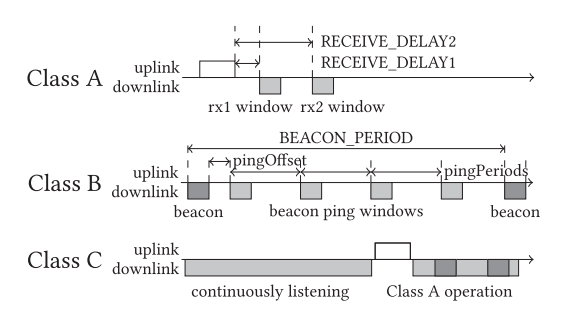
\includegraphics[scale=0.6]{figuras/ed_operations_class.png}
  \end{center}
  \legend{Fonte: \cite{hessel2023lorawan}}
\end{figure}

O LoRaWAN define três modos principais de operação para os dispositivos finais, chamados de classes A, B e C. A Classe A é a padrão e está presente em todos os dispositivos LoRaWAN. Nela, o dispositivo inicia a comunicação por meio de um \textit{uplink} e, após essa transmissão, abre duas pequenas janelas de recepção para possíveis mensagens de \textit{downlink}. Essas janelas são conhecidas como RX1 e RX2. Esse modelo é o mais eficiente em termos energéticos, pois o dispositivo permanece a maior parte do tempo fora de escuta. 

Na Classe B, além do comportamento básico da Classe A, o dispositivo sincroniza sua operação com sinais periódicos da rede e passa a abrir janelas adicionais de recepção em instantes programados. Isso permite maior previsibilidade para o envio de mensagens em \textit{downlink}, embora aumente a complexidade da operação. Já na Classe C, o dispositivo permanece praticamente em escuta contínua, fechando a recepção apenas quando transmite. Essa abordagem reduz a latência de \textit{downlink}, mas aumenta significativamente o consumo de energia, sendo mais adequada a dispositivos com menor restrição energética.

\begin{figure}[htb]
  \caption{\label{messages_abc} Estrutura e Criptografia das mensagems LoRaWan}
    \begin{center}
      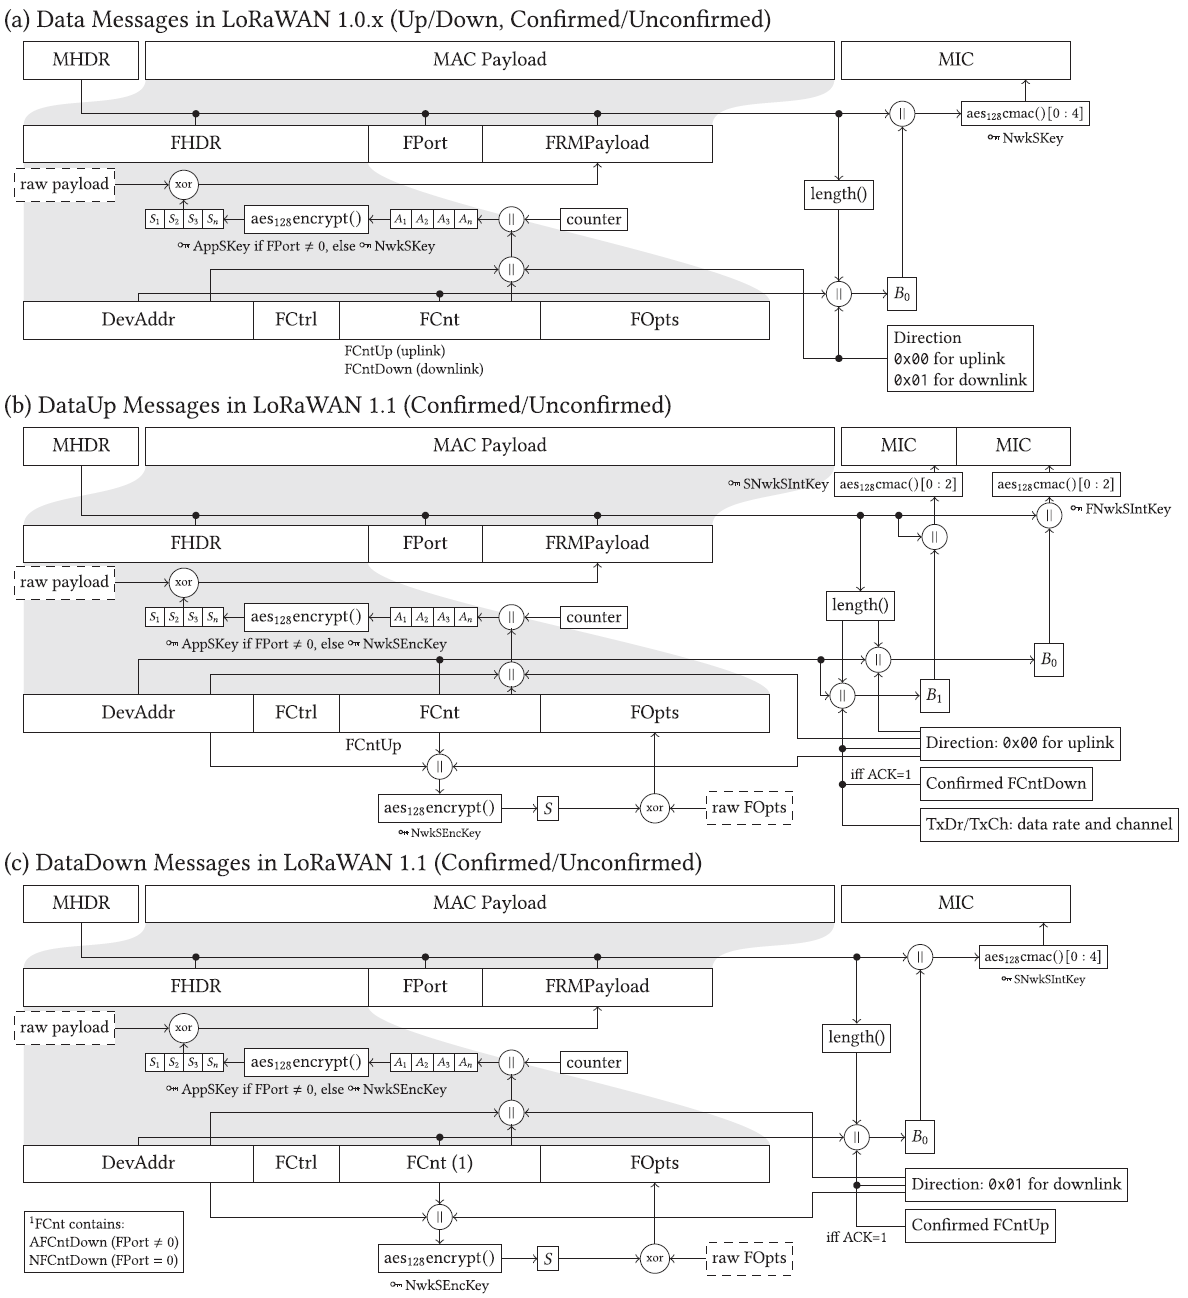
\includegraphics[scale=0.3]{figuras/structure_messages_abc.png}
  \end{center}
  \legend{Fonte: \cite{hessel2023lorawan}}
\end{figure}

As mensagens de dados do LoRaWAN possuem uma estrutura padronizada. De forma geral, elas incluem um cabeçalho com a identificação do tipo de mensagem, um cabeçalho de quadro com informações de controle e endereçamento, um contador de quadros e o campo destinado à carga útil da aplicação. Entre esses elementos, o contador de quadros, representado por \textit{FCnt}, é especialmente importante para o acompanhamento da sequência das mensagens. Outros campos, como \textit{FPort} e \textit{FOpts}, ajudam a distinguir dados de aplicação e informações de controle da rede. Além disso, as mensagens incluem um código de integridade, chamado \textit{MIC}, utilizado para verificação da validade da comunicação.

De modo geral, a transferência de dados no LoRaWAN foi projetada para equilibrar simplicidade, baixo consumo e capacidade de operação em redes distribuídas de longo alcance. A existência de diferentes classes de operação e de mecanismos para mensagens confirmadas ou não confirmadas permite adaptar o comportamento da comunicação às necessidades da aplicação. A partir dessa base, torna-se possível compreender melhor como a rede ajusta e gerencia sua operação, tema discutido na próxima subseção.

%%%%%%%%%%%%%%%%%%%%%%%%%%%%%%%%%%%%%%%%%%%%%%%%%%%%

\subsection{Gerenciamento da Rede}

Como o LoRaWAN é um protocolo de camada MAC voltado a redes LPWAN, ele precisa de mecanismos para configurar dispositivos, ajustar parâmetros de comunicação e acompanhar o estado da rede. Parte dessas funções já aparece diretamente nos próprios campos das mensagens, como endereços, contadores de quadros e confirmações. No entanto, o protocolo também define comandos específicos para gerenciamento, conhecidos como \textit{MAC commands}, que permitem trocar informações de controle entre o dispositivo final e a infraestrutura da rede. \cite{hessel2023lorawan}

Esses comandos são usados para diferentes finalidades de operação. Entre elas, estão a obtenção de informações sobre a qualidade da conexão, o ajuste de parâmetros de transmissão e a sincronização de tempo. Assim, o gerenciamento da rede não ocorre como uma função separada do restante do protocolo, mas sim como parte do próprio fluxo de comunicação entre os dispositivos e os servidores da rede. 

Entre os mecanismos de gerenciamento, um dos mais importantes é o \textit{Adaptive Data Rate} (ADR). O ADR tem como objetivo ajustar a taxa de transmissão de dados e outros parâmetros de rádio de acordo com as condições de comunicação observadas na rede. Na prática, isso permite definir combinações mais adequadas de \textit{Spreading Factor}, largura de banda e potência de transmissão, buscando equilibrar confiabilidade, consumo de energia e uso eficiente do meio de comunicação.

De forma geral, o gerenciamento da rede no LoRaWAN existe para manter a comunicação funcional e eficiente ao longo do tempo. Por meio de comandos de controle e mecanismos como o ADR, o protocolo consegue ajustar seu comportamento às condições reais de operação, o que é especialmente importante em ambientes distribuídos, sujeitos a variações de alcance, interferência e disponibilidade energética. Com essa base conceitual, torna-se possível avançar para uma análise mais voltada à forma como essas tecnologias serão utilizadas na arquitetura proposta neste trabalho.

%%%%%%%%%%%%%%%%%%%%%%%%%%%%%%%%%%%%%%%%%%%%%%%%%%%%

\subsection{LoRaWAN versus Wi-Fi no contexto do projeto}

Embora LoRaWAN e Wi-Fi sejam tecnologias de comunicação sem fio, elas atendem a necessidades diferentes e, neste trabalho, não são tratadas como soluções concorrentes. Cada uma delas ocupa um papel específico na arquitetura proposta, de acordo com suas características de alcance, consumo energético, taxa de transmissão e facilidade de integração com os demais componentes do sistema.

O LoRaWAN foi pensado para aplicações de longo alcance e baixo consumo, sendo mais adequado a dispositivos embarcados que operam com recursos limitados e transmitem pequenas quantidades de dados de forma periódica ou eventual. Essas características o tornam compatível com o cenário deste projeto, no qual os nós sensores e atuadores precisam operar de forma eficiente, com comunicação sem fio e possibilidade de instalação em locais mais afastados do ponto central da rede.

O Wi-Fi, por outro lado, oferece maior taxa de transmissão e integração mais direta com redes IP e serviços de aplicação, como APIs e servidores de armazenamento. Em contrapartida, apresenta maior consumo energético e menor adequação a nós distribuídos que precisem operar por longos períodos com restrição de energia. Por esse motivo, o Wi-Fi não foi adotado como tecnologia principal de comunicação entre os nós embarcados e a infraestrutura de campo.

No contexto deste trabalho, a solução adotada combina as duas tecnologias de forma complementar. O trecho entre os nós sensores/atuadores e o gateway utiliza LoRaWAN, preservando as vantagens de alcance e baixo consumo no nível embarcado. Já o trecho entre o gateway e o servidor utiliza Wi-Fi, aproveitando sua integração mais simples com a infraestrutura de rede e com os serviços responsáveis por receber, armazenar e processar os dados coletados.

Essa divisão permite separar dois problemas distintos dentro da arquitetura. O primeiro é a comunicação entre dispositivos embarcados em campo, em que baixo consumo e cobertura são requisitos centrais. O segundo é a entrega dos dados para uma camada de processamento e persistência, em que a prioridade passa a ser conectividade com a rede local ou com a Internet, além da facilidade de integração com a aplicação. Assim, a escolha conjunta de LoRaWAN e Wi-Fi não representa uma sobreposição de tecnologias, mas sim uma composição coerente entre camadas com funções diferentes.

Dessa forma, o uso de LoRaWAN no trecho embarcado e de Wi-Fi no trecho de retaguarda estabelece uma arquitetura compatível com os objetivos do projeto. Ao mesmo tempo em que preserva as vantagens de uma rede LPWAN na comunicação entre os dispositivos de campo, essa abordagem também facilita a construção da interface com o servidor, a persistência dos dados e a futura integração com mecanismos de análise e segurança.

%%%%%%%%%%%%%%%%%%%%%%%%%%%%%%%%%%%%%%%%%%%%%%%%%%%%

\subsection{Implicações para a arquitetura proposta}

Os conceitos apresentados nas subseções anteriores permitem situar a arquitetura adotada neste trabalho. No projeto proposto, os nós sensores e atuadores operam como dispositivos finais responsáveis pela coleta de dados do ambiente e pela transmissão dessas informações pela rede sem fio. Essa comunicação ocorre no trecho embarcado por meio do LoRaWAN, explorando suas características de longo alcance e baixo consumo energético.

O gateway exerce o papel de ponto de transição entre a rede de campo e a infraestrutura de retaguarda. Sua função principal é receber os quadros enviados pelos dispositivos finais e encaminhá-los para a camada de processamento do sistema. A partir desse ponto, os dados podem ser entregues a um servidor ou API responsável por armazenamento, organização e disponibilização das informações para etapas posteriores de análise.

Essa divisão é importante porque separa o problema da comunicação embarcada do problema de processamento dos dados. No nível dos nós em campo, o foco está em transmitir com eficiência, respeitando restrições de energia, alcance e capacidade computacional. Já no nível do gateway e do servidor, torna-se possível concentrar funções de persistência, observabilidade e integração com serviços de aplicação, sem impor esse custo diretamente aos dispositivos finais.

Entretanto, o uso do LoRaWAN por si só não elimina todos os desafios de segurança do sistema. Como discutido na literatura, a proteção efetiva da rede depende não apenas do protocolo, mas também da forma como seus mecanismos são implementados e integrados à aplicação. Em particular, a presença de dados trafegando entre dispositivos embarcados, gateway e infraestrutura de backend torna necessário considerar mecanismos adicionais de proteção, especialmente quando o sistema opera em ambientes distribuídos e sujeitos a diferentes tipos de ameaça.

Além disso, a própria dinâmica operacional da rede produz informações que podem ser úteis para análise de comportamento, identificação de falhas e detecção de atividades anômalas. Parâmetros de transmissão, padrões temporais de envio e eventos observados na comunicação podem servir como base para uma camada adicional de monitoramento do sistema, complementando a proteção oferecida pelos mecanismos tradicionais do protocolo.

Dessa forma, a arquitetura proposta neste trabalho não se limita ao transporte de dados entre dispositivos e servidor. Ela também cria as condições para incorporar camadas complementares de segurança e análise. Nesse contexto, a próxima seção discute o uso de criptografia leve como mecanismo adequado à proteção de dados em dispositivos com recursos restritos, enquanto a seção seguinte apresenta o papel do \textit{Machine Learning} como apoio à análise do comportamento da rede e à detecção de anomalias.


%%%%%%%%%%%%%%%%%%%%%%%%%%%%%%%%%%%%%%%%%%%%%%%%%%%%
%%%%%%%%%%%%%%%%%%%%%%%%%%%%%%%%%%%%%%%%%%%%%%%%%%%%

\section{Criptografia Leve (Lightweight Cryptography) e o Padrão Ascon}
Em dispositivos IoT, onde o baixo consumo de energia é um requisito essencial para viabilizar operações em diversas áreas, as aplicações que lidam com dados sensíveis e exigem sigilo demandam a adoção de métodos criptográficos que sejam, simultaneamente, leves e seguros.

O Instituto Nacional de Padrões e Tecnologia dos Estados Unidos (NIST) atua, desde 1973, no desenvolvimento de normas para proteger dados sensíveis transmitidos entre dispositivos. Seu histórico abrange desde a criação do \textit{Data Encryption Standard} (DES) e a consolidação do atual padrão de criptografia simétrica, o \textit{Advanced Encryption Standard} (AES), até as recentes padronizações de criptografia pós-quântica (\textit{Post-Quantum Cryptography}) e de criptografia leve (\textit{Lightweight Cryptography}) \cite{chen2022cornerstone}.

Com o crescimento expressivo do uso de dispositivos IoT, a necessidade de estabelecer um padrão robusto de criptografia leve tornou-se urgente. Isso impulsionou o desenvolvimento de uma nova padronização internacional com o objetivo de contemplar as primitivas criptográficas e os modos de operação adequados para ambientes restritos. Os critérios exigidos para esse novo padrão incluíam resiliência de segurança, flexibilidade de implementação, baixa sobrecarga ao integrar múltiplas funções e proteção intrínseca contra ataques de canal lateral (\textit{Side-Channel Attacks}), entre outros requisitos técnicos \cite{nistir8114}.

O processo de padronização promovido pelo NIST ocorreu ao longo de múltiplas fases de testes e escrutínio público. Inicialmente, 57 algoritmos foram submetidos para consideração. Desses, 32 avançaram para a segunda rodada e, após rigorosas avaliações de desempenho e segurança, apenas 10 chegaram à fase final. A culminação desse extenso projeto ocorreu, em 2023, com o anúncio da família Ascon como a grande vencedora \cite{ascon_official}.

O desenvolvimento do padrão Ascon começou em 2014 e ele será o foco principal deste trabalho. Na prática, ele funciona como um conjunto de algoritmos construído sob medida para dispositivos com poucos recursos. A padronização oficial conta com quatro variações principais. A primeira delas é o Ascon-AEAD128, que criptografa os dados, verifica a autenticidade da mensagem e oferece uma boa proteção contra ataques de canal lateral. A segunda variação é o Ascon-Hash256, criado especificamente para garantir a integridade dos dados transmitidos pela rede. Por fim, existem o Ascon-XOF128 e o Ascon-CXOF128. Ambos funcionam como funções de saída extensível, uma característica que permite ajustar o tamanho do \textit{hash} gerado e economizar recursos computacionais durante o processamento \cite{nist2025ascon}.

%%%%%%%%%%%%%%%%%%%%%%%%%%%%%%%%%%%%%%%%%%%%%%%%%%%%

\subsection{O Padrão Ascon-AEAD128}
O algoritmo de criptografia autenticada escolhido para o projeto pertence à família Ascon, padronizada pelo NIST sob a forma do Ascon-AEAD128 \citeonline{nist2025ascon}. Na prática, a implementação adotada neste trabalho utiliza a variante Ascon-128a, finalista do processo de padronização (versão 1.2), que compartilha a mesma estrutura de permutação do algoritmo padronizado, conforme detalhado na Seção \ref{subsec:biblioteca-ascon}. A utilização de funções de \textit{hash} adicionais não será necessária, uma vez que esse algoritmo já garante confidencialidade, integridade e autenticidade em uma única operação de criptografia autenticada.

O processo de encriptação do Ascon-AEAD128 recebe como entrada uma chave secreta e um \textit{nonce}, ambos de 128 bits, além dos dados associados (\textit{Associated Data} - AD) e o texto em claro a ser cifrado (\textit{plaintext}), que possuem tamanhos variáveis. A saída dessa função é o texto cifrado (\textit{ciphertext}) acompanhado de uma \textit{Tag} de Autenticação de 128 bits. Por sua vez, a função de decriptação recebe a chave, o \textit{nonce}, os dados associados, o texto cifrado e a \textit{tag} de autenticação. O texto original em claro só é retornado se a \textit{tag} for validada com sucesso. Caso contrário, a operação é abortada e retorna um erro (\textit{fail}).

O estado interno inicial de ambos os processos possui 320 bits, sendo formado pela concatenação de 64 bits do Vetor de Inicialização (IV), 128 bits da chave secreta e 128 bits do \textit{nonce}. Após a inicialização, o algoritmo segue em fases: primeiro ocorre o processamento dos dados associados (se presentes), seguido pela cifração do texto em blocos e, ao final de todo o processamento, a fase de finalização gera a \textit{tag} de autenticação.

\begin{figure}[htb]
  \caption{\label{fluxo-ascon-aead128-encript}Processo de encriptação do Ascon-AEAD128}
  \begin{center}
    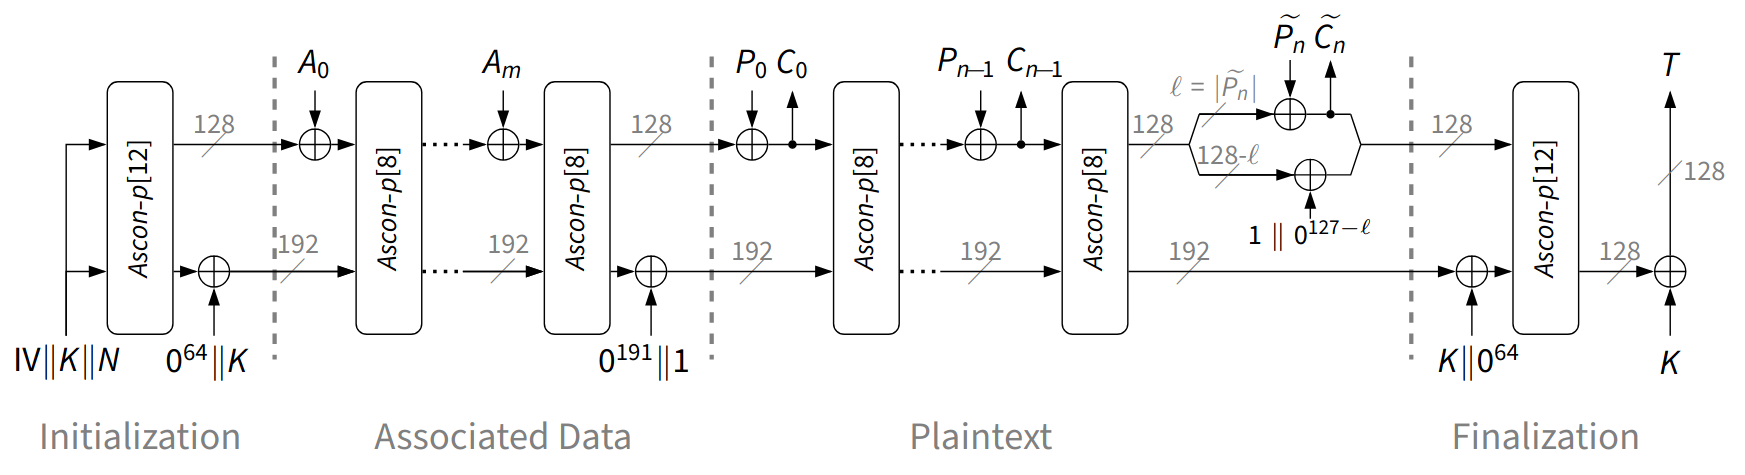
\includegraphics[scale=0.25]{figuras/fluxo-ascon-aead128-encript.png}
  \end{center}
  \legend{Fonte: \cite{nist2025ascon}}
\end{figure}

O processo de decriptação possui uma estrutura muito semelhante à da encriptação. Ele passa pela mesma inicialização do estado de 320 bits e pelo processamento dos dados associados. A diferença principal ocorre nas etapas finais: o texto cifrado é processado bloco a bloco para recuperar o texto original e, na fase de finalização, a chave secreta é combinada com o estado interno para recalcular a \textit{tag} de autenticação. Se a \textit{tag} recalculada for idêntica à \textit{tag} recebida, o texto decifrado é considerado autêntico e é retornado, caso contrário, a mensagem é descartada.

\begin{figure}[htb]
  \caption{\label{fluxo-ascon-aead128-dencript}Processo de dencriptação do Ascon-AEAD128}
  \begin{center}
    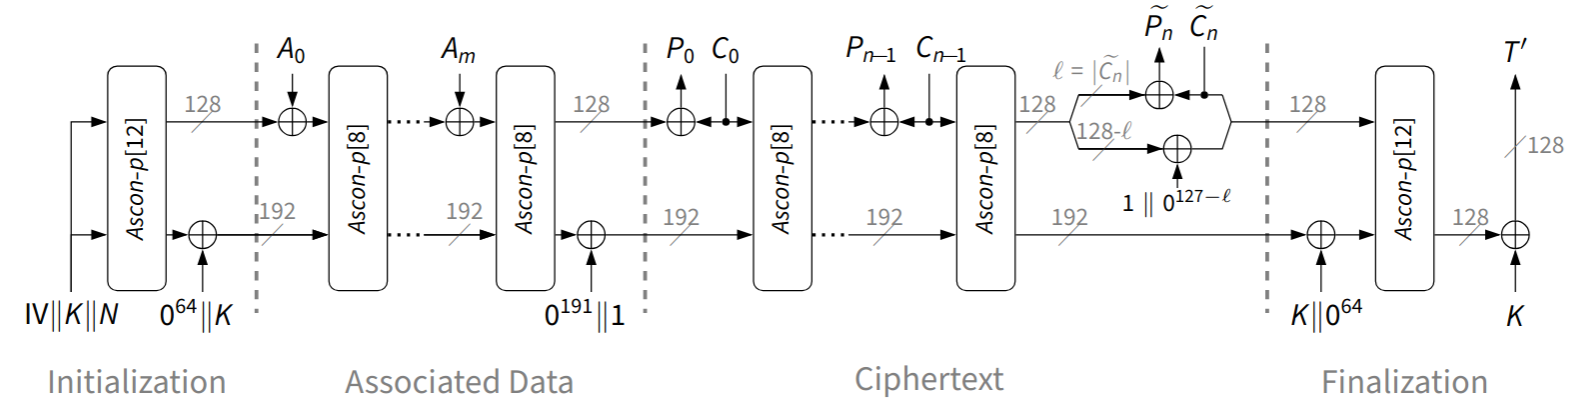
\includegraphics[scale=0.35]{figuras/fluxo-ascon-aead128-decript.png}
  \end{center}
  \legend{Fonte: \cite{nist2025ascon}}
\end{figure}

%%%%%%%%%%%%%%%%%%%%%%%%%%%%%%%%%%%%%%%%%%%%%%%%%%%%

\subsection{Comparativo de Algoritmos Criptográficos para IoT}
Durante a pesquisa inicial sobre criptografia leve, outros algoritmos foram avaliados, mas nenhum se mostrou tão adequado às necessidades do projeto quanto o padrão Ascon. Entre as principais alternativas analisadas, destacam-se o Speck \citeonline{baldi_speck} e o ChaCha20 \citeonline{bernstein2008chacha}. No entanto, a análise aprofundada revelou que nenhum destes se adequava às premissas metodológicas e práticas do projeto quanto o padrão Ascon e as soluções nativas em hardware.

O Speck é uma cifra de bloco pura e bastante leve. No entanto, ele possui uma limitação estrutural importante para redes modernas: não oferece Criptografia Autenticada com Dados Associados (\textit{AEAD}) de forma nativa. Para garantir a integridade da mensagem, seria necessária a adição de um algoritmo de autenticação secundário e independente (como um código de autenticação de mensagem, MAC). O Speck teve sua padronização internacional ativamente rejeitada pela ISO (\textit{International Organization for Standardization}) por falta de transparência em seu design \cite{register2018nsa}.

O ChaCha20, por sua vez, é uma cifra de fluxo de altíssimo desempenho, amplamente adotada como padrão da indústria para cenários de software onde \textbf{não} há aceleração de hardware disponível. Contudo, assim como o Speck, ele carece de propriedades \textit{AEAD} embutidas. A exigência extra de se acoplar o algoritmo Poly1305 consome memória e processamento. Como o microcontrolador utilizado neste trabalho (família ESP32) possui aceleração criptográfica nativa para AES, o cenário de uso principal do ChaCha20 perde o sentido prático.

Para a análise comparativa de viabilidade, este trabalho também optou por não focar nos demais algoritmos finalistas do processo de padronização do NIST (como TinyJAMBU ou Xoodyak) \citeonline{nist_lwc_finalists}, uma vez que a superioridade do Ascon sobre seus pares já foi exaustivamente documentada e comprovada pelo próprio comitê no relatório oficial NIST IR 8454 \cite{nistir8454}.

Dessa forma, a metodologia de comparação deste trabalho foi refinada para responder à questão prática sobre o embate entre o novo padrão de software e o padrão legado de hardware. Os testes focarão exclusivamente em comparar o Ascon (novo padrão \textit{Lightweight Cryptography} do NIST) contra o AES com modo de operação autenticado (\textit{AES-GCM} ou \textit{AES-CCM}) rodando diretamente no coprocessador de hardware do microcontrolador. Essa abordagem permite avaliar se a migração para a criptografia leve em software traz vantagens reais de consumo, memória e latência frente ao uso do acelerador de silício já embutido nas placas comerciais utilizadas em redes \textit{LoRaWAN}.

%%%%%%%%%%%%%%%%%%%%%%%%%%%%%%%%%%%%%%%%%%%%%%%%%%%%
%%%%%%%%%%%%%%%%%%%%%%%%%%%%%%%%%%%%%%%%%%%%%%%%%%%%

\section{Machine Learning}

O uso de \textit{Machine Learning} é coerente com o estado da arte recente. 
Trabalhos como \cite{farhad2023} demonstram que Machine Learning em 
LoRaWAN vem sendo explorado para otimizar parâmetros de rede 
(\textit{spreading factor}, potência de transmissão) e classificar padrões 
de mobilidade.

 Embora parte significativa da literatura esteja concentrada em 
desempenho e eficiência, esse mesmo conjunto de atributos também é 
extremamente relevante para tarefas de segurança e detecção de anomalias, 
já que comportamentos suspeitos frequentemente se refletem justamente em 
mudanças desses padrões operacionais \cite{farhad2023, vangelista2023}.

%%%%%%%%%%%%%%%%%%%%%%%%%%%%%%%%%%%%%%%%%%%%%%%%%%%%

\subsection{Detecção de Anomalias como Problema de Regressão Temporal}

Em redes LoRaWAN operando em condições reais, os dispositivos finais 
transmitem mensagens de forma periódica ou orientada a evento, produzindo 
naturalmente sequências de observações ao longo do tempo. Grandezas como a 
intensidade do sinal recebido, a relação sinal-ruído e os contadores de 
quadros variam de forma contínua e apresentam padrões de comportamento 
relativamente estáveis durante a operação normal da rede. Assim, desvios 
abruptos ou sistemáticos nesses padrões podem indicar a presença de falhas, 
interferências ou atividades maliciosas, tornando a análise temporal dessas 
variáveis uma abordagem promissora para a detecção de anomalias.

No entanto, a aplicação de técnicas supervisionadas de classificação enfrenta 
uma limitação estrutural importante nesse contexto. Em ambientes de operação 
real, dados rotulados que identifiquem explicitamente quadros legítimos e 
quadros associados a ataques são menos presentes.

 O \textit{dataset} Tour Perret, 
utilizado neste trabalho, é representativo da condição: trata-se de um 
conjunto de dados proveniente de sensores reais instalados na Tour Perret, 
em Grenoble, que registra o comportamento contínuo da rede sem a presença 
de rótulos de ataque. Essa característica inviabiliza a utilização direta 
de classificadores supervisionados e exige uma abordagem metodológica 
distinta - o aprendizado de padrões esperados. Mas devido a sua grande volumetria e qualidade geral de dados, esta fonte será utilizada como principal, para treinos não supervisionados, assim como descrito na seção 3.2.1.1.


A estratégia adotada neste trabalho baseia-se na modelagem do comportamento 
esperado das variáveis de rede ao longo do tempo, por meio de modelos de 
regressão para séries temporais. Nessa abordagem, o modelo é treinado 
exclusivamente sobre dados que representam a operação normal da rede, 
aprendendo os padrões temporais característicos de cada variável monitorada. Durante a fase de inferência, o modelo produz uma previsão do valor esperado 
para cada instante de tempo, e o resíduo entre o valor previsto e o valor 
observado é utilizado como indicador de anomalia. Observações cujo resíduo 
supere um limiar previamente definido (Como 3 desvios padrão da média) são sinalizadas como potencialmente 
anômalas. Esse princípio, conhecido na literatura como detecção de anomalias 
baseada em previsão, tem sido aplicado com sucesso em contextos de IoT e 
redes de sensores justamente por não depender da disponibilidade de dados 
rotulados de ataque \cite{chalapathy2019}.


\subsubsection{Contexto Prático dos Datasets Disponíveis}

A escolha da abordagem não supervisionada é também sustentada por 
limitações práticas do contexto. Para este trabalho, dois datasets 
públicos foram selecionados estrategicamente:

\begin{description}
    \item[Tour Perret (Treinamento/Validação):] Dados reais de operação 
    normal, sem injeção ou simulação de ataques. Adequado para aprender 
    padrões verdadeiros de comportamento esperado.
    
    \item[GUARD (Validação contra Ataques Conhecidos):] Dados com ataques 
    rotulados (replay, spoofing). Permite verificar se o modelo detecta 
    desvios associados a ataques já identificados.
\end{description}

Esta estratégia de dois datasets permite validação em duas fases: 
primeiro, verificar se o modelo aprendeu comportamento normal 
corretamente (Seção 3.2.3.3); segundo, verificar se detecta anomalias 
quando confrontado com ataques conhecidos (Seção 3.2.3.4). A descrição 
detalhada destes datasets é apresentada na Seção 3.2.1.


Essa escolha também apresenta uma vantagem interpretativa relevante para o 
contexto do trabalho. Ao modelar o comportamento normal da rede, torna-se 
possível não apenas detectar anomalias, mas também caracterizá-las em termos 
da magnitude e da persistência do desvio observado, oferecendo informações 
mais ricas do que uma simples classificação binária. Além disso, a abordagem 
por regressão é mais adaptável a variações graduais do comportamento da rede 
ao longo do tempo, como mudanças sazonais ou degradação natural do sinal, 
uma vez que o modelo pode ser periodicamente reatualizado com dados recentes 
de operação normal.

%%%%%%%%%%%%%%%%%%%%%%%%%%%%%%%%%%%%%%%%%%%%%%%%%%%%

\subsection{Modelos de Regressão para Séries Temporais}

A escolha dos modelos de regressão utilizados neste trabalho foi orientada 
pela necessidade de cobrir paradigmas metodológicos distintos, permitindo 
uma comparação fundamentada entre abordagens estatísticas clássicas e 
métodos baseados em aprendizado profundo. 

Nesse sentido, foram selecionados a princípio, 
três modelos: o ARIMA, a Rede Neural Recorrente simples (RNN) e a Rede de 
Memória Longa de Curto Prazo (LSTM). 

Os critérios para seleção foram:
(1) \textbf{Progressão de complexidade}: ARIMA (modelo clássico, estatístico) 
→ RNN (neural simples) → LSTM (neural com gates). Isto permite identificar 
em qual ponto a complexidade traz ganho real.
(2) \textbf{Representatividade de paradigmas}: cobrindo abordagem 
estatística, neural simples e neural avançada.
(3) \textbf{Adequação ao problema}: todos três são apropriados para séries 
temporais em IoT.
Estes pontos serão descritos com referências e de maneira mais profunda abaixo.

Outras alternativas foram consideradas (XGBoost, Prophet) mas não incluídas 
porque: XGBoost não é recorrente (inadequado para séries longas); Prophet é 
baseado em tendência, não em detecção de anomalia.

Essa progressão é metodologicamente 
importante porque permite identificar em que ponto a complexidade adicional 
do modelo se traduz em ganho efetivo de desempenho para o problema específico 
de detecção de anomalias em redes LoRaWAN.

O ARIMA (\textit{Autoregressive Integrated Moving Average}) é um modelo 
estatístico clássico amplamente utilizado para modelagem e previsão de séries 
temporais estacionárias \cite{box2015}. Sua formulação combina três 
componentes: um componente autorregressivo, que modela a dependência linear 
entre o valor atual e valores passados da série; um componente de integração, 
que torna a série estacionária por meio de diferenciação; e um componente de 
média móvel, que modela a dependência em relação aos erros de previsão 
anteriores. A principal vantagem do ARIMA neste contexto é sua 
interpretabilidade: os parâmetros do modelo têm significado estatístico 
direto e o comportamento do modelo pode ser analisado formalmente. Por esse 
motivo, o ARIMA é utilizado neste trabalho como \textit{baseline} estatístico, 
estabelecendo um patamar de referência para a avaliação dos modelos neurais 
subsequentes. Sua limitação principal reside na suposição de linearidade das 
dependências temporais, o que pode ser insuficiente para capturar padrões 
mais complexos presentes em séries de redes de sensores.

As Redes Neurais Recorrentes (RNNs) representam uma extensão natural das 
redes neurais artificiais para o domínio de sequências temporais 
\cite{rumelhart1986}. Diferentemente das redes neurais tradicionais, as RNNs 
mantêm um estado interno que é atualizado a cada instante de tempo, 
permitindo que informações de observações anteriores influenciem a previsão 
atual. Essa característica as torna adequadas para modelar dependências 
temporais sem a necessidade de especificação manual da ordem de defasagem, 
como ocorre no ARIMA. Neste trabalho, a RNN simples é utilizada como 
\textit{baseline} neural, representando o paradigma recorrente em sua forma 
mais elementar e servindo de referência para a avaliação da LSTM.

A Rede de Memória Longa de Curto Prazo (LSTM, do inglês 
\textit{Long Short-Term Memory}) é uma arquitetura recorrente desenvolvida 
especificamente para superar uma limitação fundamental das RNNs simples: o 
problema do desvanecimento do gradiente durante o treinamento 
\cite{hochreiter1997}. Em sequências longas, as RNNs tendem a perder a 
capacidade de propagar informações relevantes de instantes distantes no 
tempo, o que limita sua eficácia na modelagem de dependências temporais de 
longo alcance. A LSTM contorna esse problema por meio de uma estrutura de 
células de memória controladas por portões de entrada, esquecimento e saída, 
que regulam seletivamente quais informações devem ser retidas, atualizadas 
ou descartadas ao longo da sequência. Essa capacidade é especialmente 
relevante no contexto de redes LoRaWAN, onde padrões anômalos podem se 
manifestar como desvios sutis acumulados ao longo de múltiplos quadros 
consecutivos, e não necessariamente como eventos isolados e abruptos. Por 
esse conjunto de razões, a LSTM é tratada neste trabalho como o modelo 
principal da abordagem proposta, sendo avaliada em comparação com os dois 
\textit{baselines} anteriores.

A avaliação comparativa dos três modelos será conduzida com base em métricas 
de erro de regressão, notadamente o Erro Absoluto Médio (MAE) e a Raiz do 
Erro Quadrático Médio (RMSE), aplicadas sobre o conjunto de teste. Para a 
etapa de detecção de anomalias, o resíduo de cada modelo será submetido a 
um critério de limiarização, e o desempenho da detecção será avaliado por 
meio de métricas como precisão, revocação e taxa de falsos positivos. Essa 
distinção entre a avaliação da qualidade de previsão e a avaliação da 
capacidade de detecção é metodologicamente necessária, pois um modelo pode 
apresentar bom desempenho de regressão sem necessariamente produzir resíduos 
bem calibrados para a identificação de anomalias.

%%%%%%%%%%%%%%%%%%%%%%%%%%%%%%%%%%%%%%%%%%%%%%%%%%%%

\subsection{Considerações sobre Inferência em Dispositivos de Borda}

O treinamento e a avaliação dos modelos descritos neste trabalho são 
realizados em ambiente computacional convencional, com recursos de memória e 
processamento sem restrições relevantes. Essa decisão é adequada à fase 
atual do projeto, cujo objetivo central é investigar a eficácia das 
abordagens de detecção de anomalias antes de considerar questões de 
implantação.

No entanto, uma perspectiva relevante para a continuidade do trabalho envolve 
a possibilidade de execução do modelo treinado diretamente no gateway, 
eliminando a necessidade de transmissão dos dados brutos para uma camada 
externa de processamento. Esse paradigma, frequentemente referenciado na 
literatura como \textit{TinyML} ou inferência em borda, consiste na adaptação 
de modelos de aprendizado de máquina para execução em microcontroladores com 
severas restrições de memória RAM, armazenamento em \textit{flash} e consumo 
energético \cite{ray2022}.

A viabilidade dessa portabilidade depende fundamentalmente da complexidade do 
modelo resultante após o treinamento. Modelos com menor número de parâmetros 
e estruturas mais simples, como RNNs com poucas unidades recorrentes ou 
versões reduzidas da LSTM, são candidatos mais adequados à conversão para 
formatos otimizados de inferência, como o TensorFlow Lite for 
Microcontrollers. Técnicas adicionais de compressão, como quantização de 
pesos e poda de conexões, podem reduzir ainda mais o custo computacional sem 
perda significativa de desempenho \cite{jacob2018}.

Neste trabalho, a análise da complexidade dos modelos treinados será 
conduzida como critério complementar de avaliação, com o objetivo de fornecer 
subsídios para essa investigação futura. Contudo, a portabilidade efetiva 
para o gateway não constitui um requisito do projeto atual, sendo tratada 
como uma perspectiva de continuidade a ser explorada em trabalhos 
subsequentes, conforme discutido na Seção 7.3.



entrar no mestrado de engenharia mecânica

% Capítulo 3. Metodologia do Trabalho
\chapter{Método do trabalho} \label{cap:metodo}


Este capítulo apresenta o método adotado na construção da proposta deste trabalho. A definição da solução foi conduzida a partir de três frentes complementares: levantamento bibliográfico, análise técnica das tecnologias envolvidas e organização da arquitetura do sistema. O objetivo desse processo foi estruturar uma proposta coerente para comunicação, segurança e análise de dados em um cenário de sistemas embarcados e Internet das Coisas.

Inicialmente, é apresentada a arquitetura de comunicação e infraestrutura do sistema, que estabelece o caminho de coleta, encaminhamento e armazenamento dos dados. Em seguida, são apresentadas as etapas relacionadas à segurança e ao uso de aprendizado de máquina, consideradas como partes integradas à solução proposta. Ao final, o capítulo organiza os elementos que orientam a implementação e a avaliação do sistema.

%%%%%%%%%%%%%%%%%%%%%%%%%%%%%%%%%%%%%%%%%%%%%%%%%%%%
%%%%%%%%%%%%%%%%%%%%%%%%%%%%%%%%%%%%%%%%%%%%%%%%%%%%

\section{Procedimento de definição da arquitetura do sistema}

A definição da arquitetura do sistema foi conduzida a partir da combinação entre levantamento bibliográfico, análise técnica das tecnologias envolvidas e separação em módulos da solução proposta. O objetivo dessa etapa foi estruturar uma arquitetura coerente com o problema estudado, considerando as restrições típicas de sistemas embarcados, a necessidade de comunicação em campo e a integração posterior com mecanismos de segurança e análise.

Como referência metodológica para essa definição, o trabalho adota princípios inspirados no modelo RM-ODP, utilizando diferentes pontos de vista para organizar a solução. Em termos funcionais, foram identificados os principais blocos responsáveis pela coleta, encaminhamento, recebimento e armazenamento das informações. Em termos de informação, foram considerados os dados de aplicação e os metadados necessários para rastreabilidade, segurança e análise posterior. Em termos de engenharia, foram observadas as separações entre o trecho embarcado da comunicação, o gateway e a infraestrutura de backend.

A partir dessa organização, a arquitetura foi estruturada de modo a separar claramente a comunicação em campo da camada de aplicação. Essa separação permite tratar, de forma independente, as restrições energéticas dos nós sensores, o papel intermediário do gateway e as funções de autenticação, persistência e análise associadas ao backend. Com isso, a definição arquitetural deixa de ser apenas uma escolha de componentes e passa a refletir a distribuição de responsabilidades entre as partes do sistema.

Além da decomposição dos componentes, o procedimento de definição da arquitetura também considerou o fluxo das informações ao longo da solução. Para isso, foram analisadas as interações entre os nós de campo, o gateway e a infraestrutura de backend, buscando garantir que o sistema fosse capaz de receber, registrar e armazenar dados e metadados de forma compatível com as etapas posteriores do trabalho.

Por fim, a representação da interação entre os principais componentes foi organizada também por meio de diagramas, de modo a tornar mais clara a sequência de eventos envolvida na coleta, no encaminhamento e no armazenamento das mensagens. Essa modelagem auxilia tanto na compreensão da proposta quanto na transição entre a etapa metodológica e a etapa posterior de especificação da arquitetura.

\subsection{Critérios adotados na decomposição arquitetural}

A modularização da arquitetura foi orientada por três critérios principais. O primeiro foi a separação entre o trecho de comunicação em campo e a infraestrutura de aplicação, de modo a preservar as vantagens do uso de LoRaWAN no nível embarcado e da comunicação baseada em rede IP no nível de backend. O segundo foi a definição de responsabilidades distintas para coleta, encaminhamento, autenticação e persistência, evitando concentrar funções heterogêneas em um único componente. O terceiro foi a necessidade de manter a solução compatível com a incorporação posterior de mecanismos de criptografia leve e análise por aprendizado de máquina.

Esses critérios levaram à definição de uma arquitetura em blocos com papéis bem delimitados. No trecho embarcado, concentram-se as funções de aquisição e transmissão inicial dos dados. No ponto de transição, o gateway atua como elemento de integração entre a rede de campo e a infraestrutura de aplicação. No backend, concentram-se as funções de autenticação, persistência e preparação dos dados para uso posterior. Essa divisão favorece clareza arquitetural, reduz acoplamento entre responsabilidades e facilita a evolução incremental da solução.

\subsection{Modelagem das interações e do fluxo de dados}

Para explicitar a dinâmica de funcionamento da proposta, o fluxo principal de interação entre os componentes foi modelado em termos de sequência de eventos. Essa modelagem considera a coleta dos dados no nó de campo, a transmissão pela rede LoRaWAN, a recepção e o enriquecimento da mensagem no gateway, o encaminhamento ao backend por Wi-Fi e HTTP, e o armazenamento final de dados e metadados na infraestrutura de persistência.

A utilização de um diagrama de sequência nessa etapa é importante porque permite representar, de forma mais direta, a ordem das interações entre os componentes e os pontos em que ocorre o tratamento das mensagens. Com isso, o fluxo deixa de ser apenas uma descrição textual e passa a ser apresentado também como uma sequência organizada de ações entre entidades bem definidas.

\begin{figure}[htb]
  \caption{\label{infra_arch_1}Diagrama de sequência UML do fluxo principal}
  \begin{center}
      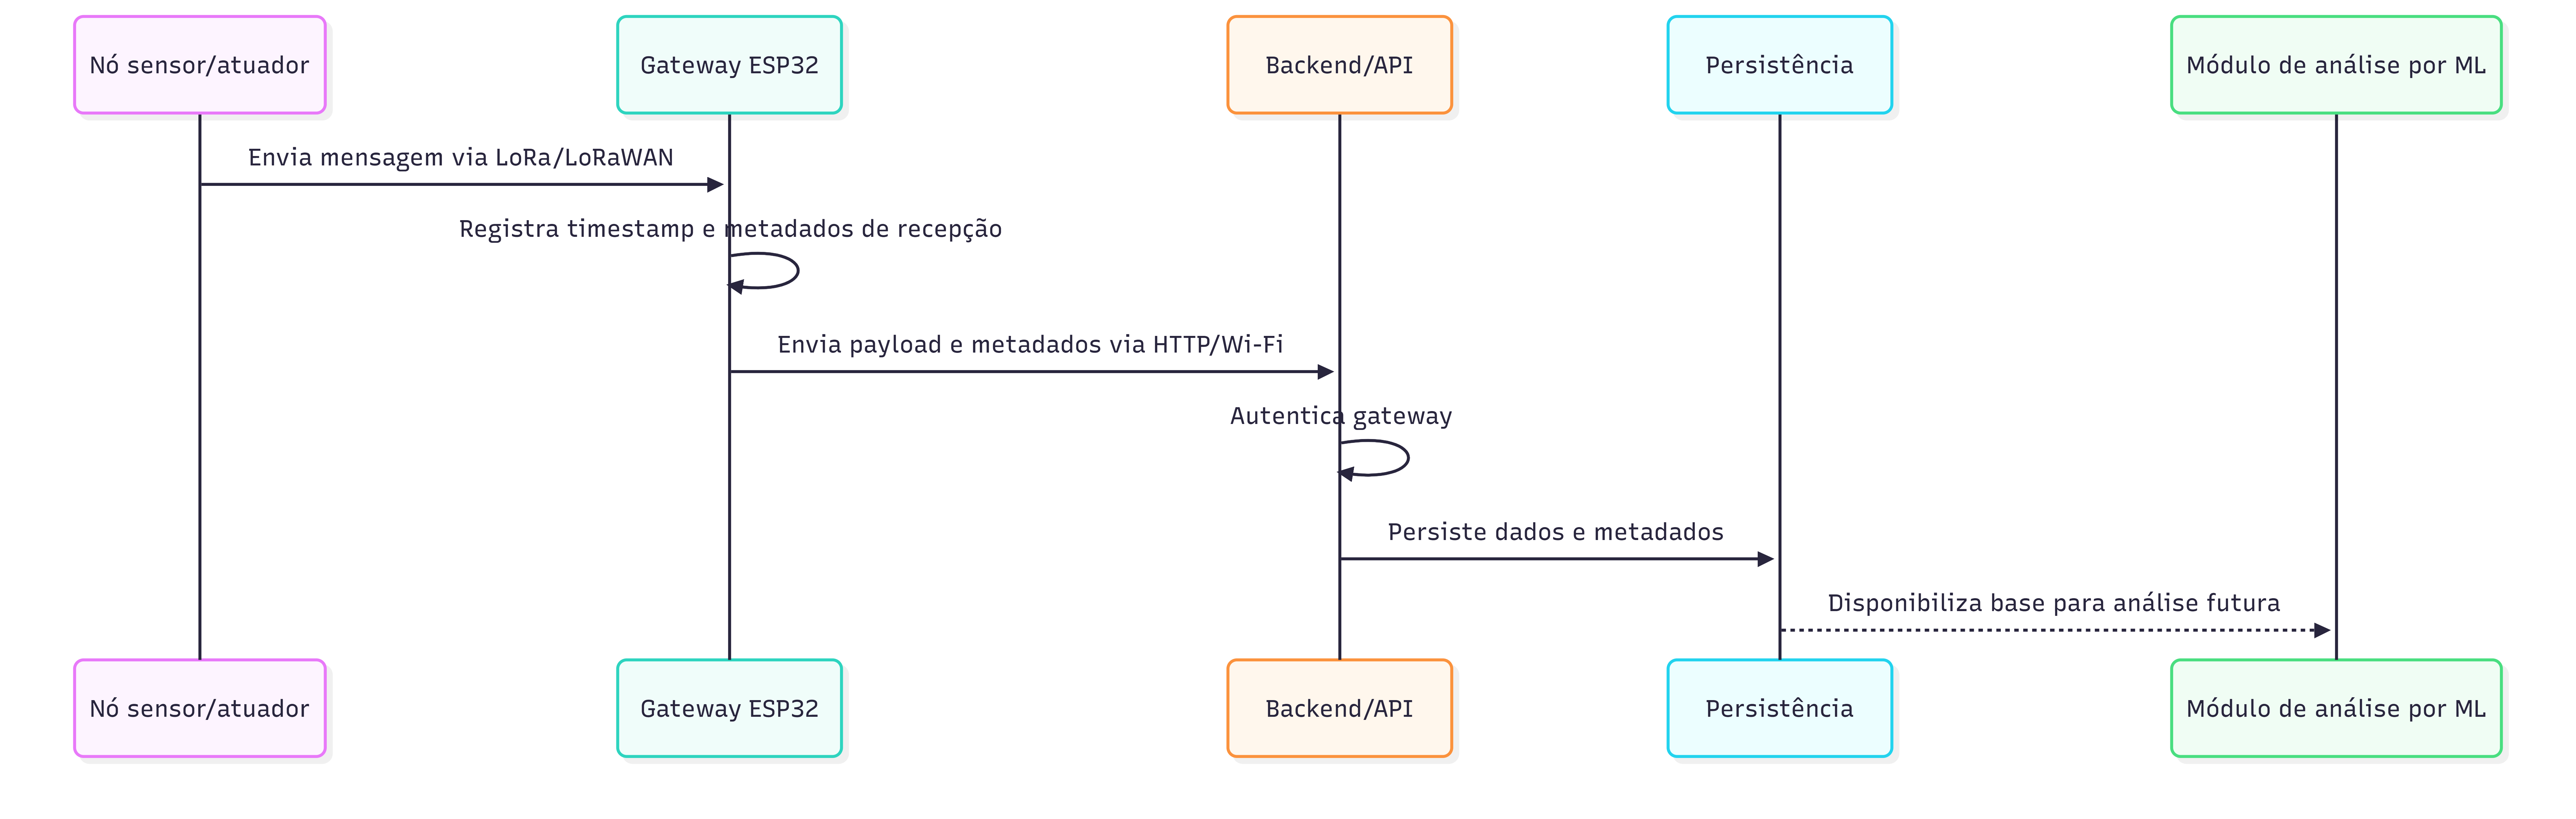
\includegraphics[scale=0.05]{figuras/arch-2-uml.png}
  \end{center}

\end{figure}

Essa representação também ajuda a evidenciar que o sistema foi concebido para operar de forma orientada a evento. Em vez de depender de comunicação contínua, o fluxo é ativado pela geração e recepção das mensagens produzidas em campo, o que torna a proposta mais compatível com o tipo de aplicação e com as restrições energéticas associadas aos dispositivos embarcados.

%%%%%%%%%%%%%%%%%%%%%%%%%%%%%%%%%%%%%%%%%%%%%%%%%%%%
%%%%%%%%%%%%%%%%%%%%%%%%%%%%%%%%%%%%%%%%%%%%%%%%%%%%

\section{Especificação de Requisitos e Revisão Bibliográfica}

%%%%%%%%%%%%%%%%%%%%%%%%%%%%%%%%%%%%%%%%%%%%%%%%%%%%
\subsection{Materiais e Bases de Dados}

Para viabilizar a etapa de modelagem, foi realizada uma pesquisa orientada 
à identificação de \textit{datasets} abertos, confiáveis e suficientemente 
completos para sustentar análises, treinamento de modelos e comparação de 
resultados. A seleção dos conjuntos de dados foi guiada por três critérios 
principais: aderência ao contexto de LoRaWAN, disponibilidade de atributos 
úteis para engenharia de \textit{features} e complementaridade entre cenários 
de operação normal e cenários com potencial presença de anomalias ou ataques.

A seleção de \textit{datasets} públicos é uma escolha orientada 
por cronograma e recursos do projeto. Pois Datasets públicos permitem focar tempo no desenvolvimento de modelos e validação 
metodológica, em vez de depender da  infraestrutura de captura. Além disso, dados 
coletados em operação real (não simulados) e já diversificados em ambiente 
real permitem comparação com outros trabalhos em literatura realizados. Por estas 
razões, foram identificados dois \textit{datasets} complementares nas 
subseções seguintes e que serão utilizados no trabalho.

%%%%%%%%%%%%%%%%%%%%%%%%%%%%%%%%%%%%%%%%%%%%%%%%%%%%

\subsubsection{Dataset Tour Perret — base principal de modelagem}

O \textit{dataset} principal adotado neste trabalho é o \textit{Tour Perret 
LoRaWAN Frames Dataset}, pertencente ao ecossistema CampusIoT. O repositório 
oficial lista o conjunto com 421.937 entradas de \textit{frames} LoRaWAN, 
coletadas a partir de dispositivos instalados na Tour Perret, em Grenoble, 
França. A plataforma CampusIoT se apresenta como uma infraestrutura de ensino 
e pesquisa voltada à experimentação \textit{in-vivo}, apoiada por uma rede 
LoRaWAN privada operando nas metrópoles de Grenoble e Valence 
\cite{campusiot_platform, tourperret_dataset}.

A principal característica que justifica a escolha desse \textit{dataset} 
como base principal é sua natureza de operação real e contínua. Os dados 
foram produzidos por sensores em funcionamento efetivo, ao longo de um 
período extenso, sem intervenção artificial no tráfego. Essa característica 
implica diretamente na ausência de rótulos de ataque, o que, longe de ser 
uma limitação, define com precisão a abordagem metodológica adequada para 
este trabalho: a modelagem do comportamento normal da rede, a partir da qual 
desvios podem ser identificados como potencialmente anômalos. Em outras 
palavras, o Tour Perret é ideal para o treinamento de modelos de regressão 
temporal voltados à detecção de anomalias não supervisionada, justamente 
porque representa com fidelidade as condições que um sistema de monitoramento 
real encontraria em campo.

Além disso, o volume de entradas do \textit{dataset} é suficiente para 
sustentar as etapas de treinamento, validação e teste com divisão temporal, 
sem comprometer a representatividade de cada partição. A diversidade de 
dispositivos e a continuidade temporal das observações também favorecem a 
construção de um modelo robusto ao comportamento variado de diferentes nós 
da rede.

%%%%%%%%%%%%%%%%%%%%%%%%%%%%%%%%%%%%%%%%%%%%%%%%%%%%

\subsubsection{Análise Exploratória do Dataset Tour Perret}

O \textit{dataset} Tour Perret foi submetido a uma análise exploratória 
preliminar com o objetivo de caracterizar sua estrutura, verificar a 
qualidade dos dados disponíveis e identificar os atributos mais relevantes 
para a etapa de modelagem. Essa análise constitui parte integrante do método 
adotado, fornecendo evidências concretas que embasam as decisões de seleção 
de variáveis descritas na Seção~\ref{sec:selecao_variaveis}.

O conjunto de dados é composto por 421.937 entradas de \textit{frames} 
LoRaWAN, distribuídas entre três cenários identificados pelo campo 
\texttt{applicationName}: o cenário \texttt{ELSYS\_EMS}, predominante com 
412.380 registros (97,7\% do total), o cenário \texttt{WYRES\_BASE}, com 
9.526 registros, e um terceiro identificador com 31 entradas. Essa 
concentração em um único cenário de aplicação é metodologicamente favorável, 
pois permite que a modelagem do comportamento normal seja construída sobre 
uma base homogênea, reduzindo a influência de padrões heterogêneos entre 
aplicações distintas.

A verificação de cobertura dos campos revelou alta qualidade dos dados para 
todos os atributos relevantes ao projeto, conforme apresentado na 
Tabela~\ref{tab:cobertura_tourperret}. Os campos \texttt{timestamp}, 
\texttt{devEUI} e \texttt{rxInfo} apresentaram preenchimento de 100\%, 
enquanto \texttt{fCnt}, \texttt{fPort} e \texttt{\_redundancy} atingiram 
99,99\%, e o campo \texttt{object}, que contém o \textit{payload} 
decodificado, registrou 99,98\% de preenchimento. Essa consistência indica 
que o \textit{dataset} é adequado para o treinamento de modelos de regressão 
temporal sem necessidade de estratégias complexas de imputação de dados 
ausentes.

\begin{table}[htb]
\centering
\caption{Cobertura dos campos relevantes no dataset Tour Perret}
\label{tab:cobertura_tourperret}
\begin{tabular}{lll}
\hline
\textbf{Atributo} & \textbf{Campo original} & \textbf{Preenchimento (\%)} \\
\hline
timestamp    & \texttt{\_timestamp}  & 100,00 \\
device\_id   & \texttt{devEUI}       & 100,00 \\
gateway\_info & \texttt{rxInfo}      & 100,00 \\
fCnt         & \texttt{fCnt}         & 99,99  \\
freq\_dr     & \texttt{txInfo}       & 100,00 \\
fPort        & \texttt{fPort}        & 99,99  \\
payload      & \texttt{object}       & 99,98  \\
redundância  & \texttt{\_redundancy} & 99,99  \\
\hline
\end{tabular}
\legend{Fonte: elaborado pelos autores.}
\end{table}

A análise de diversidade identificou 5 dispositivos únicos no subconjunto 
analisado, com distribuição heterogênea de volume de mensagens entre eles. 
A variabilidade de RSSI por dispositivo foi calculada e revelou perfis 
distintos de enlace para cada nó da rede, conforme apresentado na 
Tabela~\ref{tab:rssi_dispositivos}. O dispositivo \texttt{42fb8334...} 
apresentou o maior desvio padrão de RSSI (11,30 dBm), indicando condições 
de enlace mais instáveis, enquanto o dispositivo \texttt{73d89239...} exibiu 
o menor desvio (5,83 dBm), sugerindo um enlace mais estável ao longo do 
tempo. As médias de RSSI variaram entre $-$97,38 dBm e $-$107,76 dBm entre 
os dispositivos, confirmando que o perfil de sinal é característico de cada 
nó e potencialmente utilizável como base para a modelagem de comportamento 
esperado individualizado.

\begin{table}[htb]
\centering
\caption{Variabilidade de RSSI por dispositivo no dataset Tour Perret}
\label{tab:rssi_dispositivos}
\begin{tabular}{lrrrr}
\hline
\textbf{devEUI (parcial)} & \textbf{Média (dBm)} & \textbf{Desvio padrão} & 
\textbf{Mín} & \textbf{Máx} \\
\hline
2951cd7c... & $-$106,43 & 6,76  & $-$127 & $-$59 \\
42fb8334... & $-$97,38  & 11,30 & $-$122 & $-$74 \\
441a1ed9... & $-$103,45 & 9,01  & $-$127 & $-$76 \\
73d89239... & $-$107,76 & 5,83  & $-$126 & $-$68 \\
73fe90c2... & $-$103,64 & 10,02 & $-$130 & $-$55 \\
\hline
\end{tabular}
\legend{Fonte: elaborado pelos autores.}
\end{table}

As \textit{features} numéricas RSSI, SNR, frequência de operação e 
\textit{data rate} foram extraídas com sucesso das estruturas aninhadas dos 
campos \texttt{rxInfo} e \texttt{txInfo}, confirmando a viabilidade de 
utilização desses atributos nos modelos de regressão. O fato de que essas 
variáveis estão disponíveis de forma consistente em praticamente todas as 
entradas do \textit{dataset} reforça sua adequação como candidatas principais 
à seleção final de variáveis, discutida na 
Seção~\ref{sec:selecao_variaveis}.

Em conjunto, os resultados da análise exploratória confirmam que o 
\textit{dataset} Tour Perret apresenta qualidade, volume e riqueza de 
atributos suficientes para sustentar a etapa de modelagem proposta neste 
trabalho, tanto em termos de dados de treinamento quanto de variáveis 
candidatas para a construção dos modelos de regressão temporal.

%%%%%%%%%%%%%%%%%%%%%%%%%%%%%%%%%%%%%%%%%%%%%%%%%%%%

\subsubsection{Dataset GUARD — papel complementar e de referência}

O segundo \textit{dataset} considerado neste trabalho é o 
\textit{LoRaWAN Network Attacks}, associado ao projeto GUARD. De acordo com 
sua descrição oficial, esse conjunto contém um \textit{dump} de mensagens 
observadas em uma rede LoRaWAN durante a validação do projeto, incluindo 
tráfego legítimo proveniente de dispositivos reais instalados em ônibus 
urbanos, além de ataques artificialmente gerados por replicação ou alteração 
de mensagens \cite{guard_dataset}.

%%%%%%%%%%%%%%%%%%%%%%%%%%%%

\paragraph{Caracterização dos Ataques em GUARD}

Uma análise exploratória do \textit{dataset} GUARD foi conduzida para 
caracterizar a natureza dos ataques contidos. Embora o \textit{dataset} 
não forneça rótulos explícitos (coluna binária de ataque/normal), contém 
indicadores comportamentais estruturados que permitem identificação 
confiável de eventos anômalos.

A análise focou nas colunas \texttt{type} e \texttt{error}, que registram 
eventos durante processamento de mensagens LoRaWAN. Foram identificados dois 
indicadores principais:

\begin{enumerate}
    \item \textbf{UPLINK\_FCNT\_RETRANSMISSION}: Frame counter não incrementou 
    sequencialmente, indicando retransmissão de mensagem anterior (ataque de 
    replicação).
    
    \item \textbf{UPLINK\_FCNT\_RESET}: Frame counter sofreu reset inesperado, 
    indicando contador adulterado ou dispositivo comprometido (ataque de 
    spoofing).
\end{enumerate}

A filtragem sistemática identificou \textbf{6.799 registros} com um ou mais 
destes indicadores, representando eventos anômalos confirmados. Esta 
quantidade significativa fornece volume adequado para validação de capacidade 
de detecção.

%%%%%%%%%%%%%%%%%%%%%%%

\paragraph{Estratégias de Validação com GUARD}

Diferentemente do Tour Perret, o \textit{dataset} GUARD contém indicadores 
de ataque explicitamente identificáveis através de suas colunas 
\texttt{type} e \texttt{error}. No contexto deste trabalho, contudo, ele 
exerce um papel complementar e não central, sendo utilizado em duas 
estratégias de validação distintas.

\subparagraph{Estratégia 1: Teste de Generalização}

Após treinar o modelo com Tour Perret (aprendendo padrões de comportamento 
normal), aplicar este modelo aos dados de GUARD para verificar se consegue 
identificar desvios associados a ataques conhecidos. Esta abordagem responde 
à questão: \textit{``O modelo consegue detectar anomalias mesmo quando 
confrontado com contexto diferente daquele em que foi treinado?''}

Importa notar que esta validação possui uma limitação intrínseca: Tour 
Perret (sensores em Grenoble) e GUARD (ônibus urbanos) representam 
contextos distintos. Portanto, quando o modelo detecta desvios em GUARD, 
isto pode resultar tanto de (i) identificação de ataque quanto de 
(ii) mudança de contexto ambiental. Assim, esta abordagem valida 
\textit{sensibilidade} do modelo a anomalias, mas não isoladamente a 
capacidade de distinguir ataques de mudanças contextuais.

\subparagraph{Estratégia 2: Validação Supervisionada (Se Viável)}

Se análise mais profunda de GUARD indicar viabilidade, uma segunda 
estratégia envolve treinar um classificador supervisionado (Normal vs 
Ataque) exclusivamente dentro de GUARD, usando os 6.799 registros anômalos 
como ``ataque'' e registros restantes como ``normal''. Validação cruzada 
dentro de GUARD forneceria comparação direta com a abordagem não 
supervisionada de Tour Perret.

Esta estratégia enfrenta dois desafios práticos reconhecidos:

\begin{enumerate}
    \item \textbf{Engenharia de features}: Campos estruturados de GUARD 
    (\texttt{time}, \texttt{tx\_info}, \texttt{rx\_info}, \texttt{data}) 
    requerem transformação significativa em features numéricas compatíveis 
    com modelos de aprendizado de máquina, consumindo tempo de 
    desenvolvimento.
    
    \item \textbf{Desbalanceamento de classes}: O \textit{dataset} GUARD 
    possui proporção desigual entre registros normais e registros de ataque. 
    Treinar modelos supervisionados com desbalanceamento severo introduz 
    viés. Técnicas de balanceamento (oversampling, undersampling, pesos de 
    classe) seriam necessárias.
\end{enumerate}

Por estas razões, a abordagem supervisionada é considerada secundária e 
explorada apenas se cronograma permitir. Do contrário, será considerada uma perspectiva de continuidade, como futuros passos.

\subparagraph{Objetivos Distintos, Insights Complementares}

As duas estratégias respondem a questões metodologicamente diferentes:

\begin{enumerate}
    \item \textbf{Tour Perret (Não Supervisionado)}: ``O modelo consegue 
    aprender padrões normais e detectar desvios significativos?'' Fornece 
    validação da abordagem de regressão temporal em dados reais de operação 
    normal.
    
    \item \textbf{GUARD - Generalização}: ``O modelo generaliza para novo 
    contexto?'' Fornece indicação de robustez do modelo a variações ambientais.
    
    \item \textbf{GUARD - Supervisionado} (se viável): ``O modelo consegue 
    classificar quando dispõe de rótulos explícitos?'' Fornece comparação 
    com baseline supervisionado.
\end{enumerate}

A combinação destas estratégias enriquece a análise sem exigir que o modelo 
principal seja treinado exclusivamente com dados rotulados, mantendo o 
cronograma viável.

%%%%%%%%%%%%%%%%%%%%%%%%%%%%%%%%%%%%%%%%%%%%%%%%%%%%

\subsection{Seleção de Variáveis}
\label{sec:selecao_variaveis}

A definição das variáveis de entrada dos modelos de regressão é uma etapa 
metodológica central neste trabalho, pois determina diretamente quais 
aspectos do comportamento da rede serão modelados e, consequentemente, quais 
tipos de anomalia o sistema será capaz de detectar. A seleção foi conduzida 
a partir de dois critérios principais: relevância para a caracterização do 
comportamento temporal da rede LoRaWAN e disponibilidade consistente nos 
\textit{datasets} selecionados.

O \textit{dataset} Tour Perret disponibiliza um conjunto de atributos 
associados a cada \textit{frame} recebido, entre os quais se destacam como 
candidatos naturais à modelagem temporal as seguintes variáveis: a 
intensidade do sinal recebido (RSSI), a relação sinal-ruído (SNR), o 
contador de \textit{frames} (FCnt), o intervalo de tempo entre mensagens 
consecutivas de um mesmo dispositivo (\textit{inter-arrival time}) e a taxa 
de dados utilizada na transmissão (\textit{data rate}). Cada uma dessas 
variáveis apresenta propriedades distintas do ponto de vista da detecção de 
anomalias.

O RSSI e o SNR refletem as condições do enlace de rádio e tendem a variar 
de forma gradual em condições normais de operação. Variações abruptas nesses 
indicadores podem sinalizar interferência deliberada, mudança de posição do 
dispositivo ou substituição fraudulenta de um nó — padrões associados a 
ataques de \textit{jamming} e \textit{spoofing}, respectivamente. O FCnt, 
por sua vez, deve apresentar incremento monotônico e regular ao longo do 
tempo para um dispositivo legítimo. Quebras nesse padrão, como saltos 
inesperados ou regressões no contador, são características típicas de 
ataques de \textit{replay}, nos quais mensagens anteriores são 
retransmitidas por um adversário. O \textit{inter-arrival time} captura o 
ritmo de transmissão do dispositivo e é especialmente sensível a 
comportamentos de \textit{flooding} ou a tentativas de esgotamento do 
canal \cite{hessel2023lorawan}. O \textit{data rate}, embora ajustado 
dinamicamente pelo mecanismo ADR, também pode apresentar variações anômalas 
em situações de interferência ou manipulação da comunicação.

A seleção final das variáveis a serem utilizadas nos modelos será definida 
com base na análise exploratória dos dados do Tour Perret descrita na 
Seção~3.2.1.2, considerando a estabilidade temporal de cada atributo, a 
presença de valores ausentes e a correlação entre variáveis candidatas. O 
objetivo é identificar um subconjunto reduzido — preferencialmente de até 
três variáveis — que concentre o maior poder explicativo para a modelagem do 
comportamento normal da rede, mantendo a complexidade do modelo compatível 
com uma eventual análise de portabilidade futura para dispositivos de borda.

%%%%%%%%%%%%%%%%%%%%%%%%%%%%%%%%%%%%%%%%%%%%%%%%%%%%

\subsection{Procedimentos de Treinamento e Avaliação}

O treinamento dos modelos de regressão será realizado em ambiente 
computacional convencional, sem restrições relevantes de memória ou 
processamento. Essa decisão é adequada à fase atual do projeto, cujo 
objetivo é avaliar a eficácia das abordagens de detecção de anomalias antes 
de qualquer consideração sobre implantação em dispositivos restritos.

%%%%%%%%%%%%%%%%%%%%%%%%%%%%%%%%%%%%%%%%%%%%%%%%%%%%

\subsubsection{Preparação e Divisão dos Dados}

Antes do treinamento, os dados do Tour Perret serão submetidos a uma etapa 
de preparação que inclui harmonização de \textit{timestamps}, tratamento de 
valores ausentes, normalização das variáveis selecionadas e organização das 
sequências por dispositivo. A divisão dos dados entre conjuntos de 
treinamento, validação e teste seguirá uma lógica de divisão temporal 
(\textit{temporal split}), na qual as observações mais antigas compõem o 
conjunto de treinamento e as mais recentes compõem os conjuntos de validação 
e teste. Essa abordagem é metodologicamente necessária para séries temporais, 
pois preserva a ordem cronológica dos dados e evita o vazamento de informação 
futura para o treinamento (\textit{data leakage}), problema que ocorreria em 
divisões aleatórias \cite{bergmeir2012, hyndman2021}.

%%%%%%%%%%%%%%%%%%%%%%%%%%%%%%%%%%%%%%%%%%%%%%%%%%%%

\subsubsection{Treinamento dos Modelos}

Os três modelos descritos na Seção~2.3.2 — ARIMA, RNN e LSTM — serão 
treinados sobre o conjunto de treinamento, exclusivamente com dados que 
representam a operação normal da rede. Para o ARIMA, a ordem dos componentes 
autorregressivo, de integração e de média móvel será determinada por meio de 
análise das funções de autocorrelação e autocorrelação parcial da série 
\cite{box2015}. Para a RNN e a LSTM, a arquitetura das redes será definida 
de forma a manter o número de parâmetros em um nível compatível com a 
complexidade do problema, favorecendo a generalização e a eventual análise 
de portabilidade.

%%%%%%%%%%%%%%%%%%%%%%%%%%%%%%%%%%%%%%%%%%%%%%%%%%%%

\subsubsection{Avaliação da Qualidade de Regressão}

A qualidade de previsão de cada modelo será avaliada sobre o conjunto de 
teste por meio do Erro Absoluto Médio (MAE) e da Raiz do Erro Quadrático 
Médio (RMSE). Essas métricas quantificam a magnitude média dos erros de 
previsão, sendo o RMSE mais sensível a erros grandes e pontuais, e o MAE 
mais robusto a \textit{outliers} \cite{hyndman2021}.


Formalmente, o Erro Absoluto Médio é calculado como:

\[
\mathrm{MAE} = \frac{1}{n} \sum_{i=1}^{n} |y_i - \hat{y}_i|
\]

e a Raiz do Erro Quadrático Médio é:

\[
\mathrm{RMSE} = \sqrt{\frac{1}{n} \sum_{i=1}^{n} (y_i - \hat{y}_i)^2}
\]

em que $n$ é o número de observações no conjunto de teste, $y_i$ é o 
valor observado e $\hat{y}_i$ é o valor previsto pelo modelo no instante $i$.

O MAE mede o erro médio em termos absolutos, oferecendo interpretação 
direta na unidade da variável. O RMSE, ao elevar os erros ao quadrado 
antes da média, penaliza mais fortemente erros grandes, tornando-o mais 
sensível a \textit{outliers}. Assim, o MAE é mais robusto a anomalias 
pontuais, enquanto o RMSE fornece indicação de quão grave são os erros 
de previsão quando ocorrem.

%%%%%%%%%%%%%%%%%%%%%%%%%%%%%%%%%%%%%%%%%%%%%%%%%%%%

\subsubsection{Avaliação da Capacidade de Detecção de Anomalias}

A etapa de detecção de anomalias é conduzida de forma independente da 
avaliação de regressão, pois um modelo com bom desempenho de previsão não 
produz necessariamente resíduos bem calibrados para a identificação de 
desvios \cite{chalapathy2019}. O procedimento consiste em calcular o resíduo 
entre o valor previsto e o valor observado para cada instante do conjunto de 
teste e aplicar um critério de limiarização para classificar cada observação 
como normal ou potencialmente anômala. O limiar será definido com base na 
distribuição dos resíduos observados no conjunto de validação, adotando como 
referência um múltiplo do desvio padrão dos erros de treinamento.

Para a avaliação da detecção, serão utilizadas métricas de classificação 
binária, incluindo precisão, revocação e taxa de falsos positivos. No 
contexto de segurança em redes IoT, a revocação — isto é, a capacidade do 
modelo de identificar corretamente eventos anômalos — é a métrica de maior 
relevância operacional, pois falhas na detecção de ataques reais têm 
consequências mais graves do que a geração de alarmes falsos \cite{hessel2023lorawan}. 
A taxa de falsos positivos, por sua vez, é igualmente importante do ponto de 
vista da operabilidade do sistema, uma vez que um número elevado de alarmes 
incorretos pode comprometer a confiança e a utilidade prática da solução.

%%%%%%%%%%%%%%%%%%%%%%%%%%%%%%%%%%%%%%%%%%%%%%%%%%%%

\subsection{Procedimentos de Treinamento e Avaliação}
A implementação da abordagem de \textit{Machine Learning} foi concebida a partir da hipótese de que anomalias em redes LoRaWAN podem ser identificadas por meio de desvios em padrões temporais, atributos de enlace e características do tráfego observado. Com base nisso, a estratégia de modelagem foi estruturada em etapas sucessivas: inspeção e padronização dos dados, seleção e engenharia de atributos, treinamento de modelos, comparação entre abordagens e análise dos resultados.

Na etapa de preparação dos dados, torna-se necessário harmonizar \textit{timestamps}, normalizar identificadores de dispositivos e \textit{gateways}, tratar campos ausentes e organizar atributos comuns entre datasets distintos. Em seguida, são construídas variáveis de entrada que representem tanto o estado instantâneo do \textit{frame} quanto seu contexto temporal. Entre os atributos mais relevantes para essa análise, destacam-se métricas como RSSI, SNR, frequência de operação, \textit{data rate}, presença de redundância de recepção, progressão de \textit{frame counters}, intervalo entre mensagens e padrões de repetição de \textit{payload} ou comportamento por dispositivo.

A modelagem pode então ser conduzida por duas frentes complementares. A primeira envolve métodos voltados à detecção de anomalias com pouca ou nenhuma dependência de rótulos completos, o que é particularmente útil em cenários reais de IoT. A segunda envolve, quando houver suporte suficiente dos dados, experimentos comparativos com métodos supervisionados ou semi-supervisionados, sobretudo nos casos em que o dataset apresenta descrição de tráfego manipulado ou cenários de ataque. Essa combinação é apropriada porque permite comparar não apenas acurácia bruta, mas também robustez metodológica diante de diferentes qualidades de rotulação.

Além disso, a estratégia adotada considera que a utilidade dos modelos não deve ser avaliada apenas em função do desempenho estatístico, mas também em relação à sua compatibilidade com execução futura em dispositivos restritos. Por esse motivo, o desenvolvimento da modelagem já considera a complexidade dos métodos, o número de atributos utilizados e o custo potencial de inferência, buscando favorecer posteriormente sua adaptação para contextos de borda. 

%%%%%%%%%%%%%%%%%%%%%%%%%%%%%%%%%%%%%%%%%%%%%%%%%%%%

\subsection{Biblioteca Ascon}
\label{subsec:biblioteca-ascon}
Para a implementação das primitivas criptográficas no microcontrolador, optou-se pela utilização da biblioteca de código aberto \textit{ascon-suite}, mantida por \citeonline{weatherley2023ascon}. A escolha desta implementação específica, em detrimento do repositório de referência matemático original (\textit{ascon-c}), justifica-se por fatores arquiteturais estritamente alinhados aos objetivos de prototipagem em sistemas embarcados.

Primeiramente, a \textit{ascon-suite} foi estruturada com foco em plataformas com restrição de recursos, fornecendo rotinas de \textit{backend} altamente otimizadas em linguagem \textit{Assembly}, podendo ser usada diretamente na IDE do Arduino como uma biblioteca, facilitando o desenvolvimento na placa ESP32.

Em segundo lugar, a biblioteca expõe uma Interface de Programação de Aplicações (API) de alto nível que suporta processamento de dados de forma incremental. Essa característica permite a criptografia de fluxos e \textit{payloads} em pequenos fragmentos, o que é um recurso imperativo para garantir que o microcontrolador não esgote sua limitada memória RAM ao tentar alocar mensagens inteiras de uma só vez antes da transmissão via rádio.

Por fim, o rigor técnico da biblioteca possui forte validação científica. Os códigos otimizados em \textit{Assembly} e C que deram origem à \textit{ascon-suite} foram ativamente empregados como base metodológica para a extração de métricas de desempenho em microcontroladores durante o processo de padronização do NIST, tendo seus resultados oficialmente documentados na seção 4.1.3 do relatório governamental NIST IR 8454 \cite{nistir8454}.

A implementação utilizada neste trabalho, fornecida pela biblioteca ascon-suite, corresponde à versão finalista submetida à competição de Criptografia Leve do NIST (Ascon v1.2), e não à forma normatizada posteriormente na publicação SP 800-232 (2025). Especificamente, adota-se a variante Ascon-128a, que compartilha a mesma estrutura de permutação do Ascon-AEAD128 padronizado. As diferenças entre a v1.2 e o SP 800-232 restringem-se ao vetor de inicialização, à ordenação de bytes na interface de entrada/saída e à separação de domínio. Como o custo computacional do Ascon é dominado pelas aplicações da permutação, idênticas nas duas versões, espera-se que as métricas de desempenho, memória e energia sejam essencialmente equivalentes.

%%%%%%%%%%%%%%%%%%%%%%%%%%%%%%%%%%%%%%%%%%%%%%%%%%%%
%%%%%%%%%%%%%%%%%%%%%%%%%%%%%%%%%%%%%%%%%%%%%%%%%%%%

\section{Atividades propostas para desenvolvimento e validação}

As atividades propostas nesta etapa do trabalho foram organizadas de modo a permitir a evolução progressiva da solução, partindo da infraestrutura básica de comunicação e avançando, posteriormente, para a incorporação das camadas de segurança e análise. Essa organização busca reduzir a complexidade da integração inicial e tornar mais clara a relação entre os diferentes módulos do sistema ao longo do desenvolvimento do projeto.

%%%%%%%%%%%%%%%%%%%%%%%%%%%%%%%%%%%%%%%%%%%%%%%%%%%%

\subsection{Integração progressiva da infraestrutura}

A primeira frente de atividade considera a integração da infraestrutura básica de comunicação, envolvendo os nós de campo, o gateway e a camada de backend. Nessa etapa, o foco está no estabelecimento do fluxo principal do sistema, de modo que os dados produzidos em campo possam ser recebidos, encaminhados, autenticados e armazenados de forma consistente.

Em seguida, a proposta considera a consolidação da persistência dos dados e metadados gerados ao longo da comunicação. Essa base é necessária não apenas para o funcionamento da solução, mas também para dar suporte às etapas seguintes do trabalho. Após essa consolidação, passam a ser incorporadas as atividades relacionadas à proteção criptográfica dos dados e à exploração analítica das informações persistidas.

%%%%%%%%%%%%%%%%%%%%%%%%%%%%%%%%%%%%%%%%%%%%%%%%%%%%

\subsection{Atividades propostas de validação}

As atividades de validação previstas no trabalho acompanham a evolução da integração da solução. Inicialmente, será observada a consistência do fluxo de comunicação entre os dispositivos de campo, o gateway e o backend. Em seguida, serão consideradas atividades voltadas ao registro correto de metadados, à persistência das informações e ao comportamento do sistema em situações de falha temporária de conectividade.

Em etapas posteriores, a validação passa a incluir a incorporação da camada criptográfica baseada em Ascon e o uso da base persistida em análises por aprendizado de máquina. Com isso, a avaliação deixa de incidir apenas sobre a comunicação básica e passa a contemplar também o comportamento integrado da proposta, reunindo infraestrutura, segurança e análise de dados.

%%%%%%%%%%%%%%%%%%%%%%%%%%%%%%%%%%%%%%%%%%%%%%%%%%%%

\subsection{Relação com o cronograma do projeto}

A organização dessas atividades em etapas também tem a função de alinhar a evolução técnica da solução ao cronograma do projeto. Em um primeiro momento, concentram-se os esforços na definição e integração da infraestrutura básica. Em seguida, a continuidade do trabalho contempla a inserção progressiva das demais frentes, de modo que a arquitetura possa ser avaliada em níveis crescentes de complexidade.

Essa organização permite que cada etapa produza uma base para a etapa seguinte, reduzindo retrabalho e favorecendo a coerência do desenvolvimento como um todo. Dessa forma, o cronograma deixa de ser apenas uma divisão temporal de tarefas e passa a refletir a lógica de construção incremental da proposta.

%%%%%%%%%%%%%%%%%%%%%%%%%%%%%%%%%%%%%%%%%%%%%%%%%%%%
%%%%%%%%%%%%%%%%%%%%%%%%%%%%%%%%%%%%%%%%%%%%%%%%%%%%

\section{Testes e Avaliação de Desempenho (\textit{Benchmarking})}
\label{subsec:validacao-ascon}
\subsection{\textit{Known Answer Tests} (KAT)}
A primeira etapa será a validação através dos \textit{Known Answer Tests} (KAT), que são testes disponibilizados pelo próprio grupo que desenvolveu o Ascon. Eles fornecem parâmetros de entrada específicos que devem resultar em saídas exatas e já esperadas. Como o trabalho utiliza a variante Ascon-128a (versão 1.2), a validação emprega os vetores de teste correspondentes a essa versão, distribuídos junto à própria \textit{ascon-suite} e derivados do repositório de referência \textit{ascon-c} \cite{ascon_reference_c}.

Para validar a biblioteca de forma puramente matemática, os testes serão rodados exaustivamente em um computador desktop. Depois, para garantir que não haja nenhuma anomalia de compilação ou diferença causada pela arquitetura de hardware, testes adicionais serão executados diretamente na placa, mas com um volume menor de vetores.

Como garantia extra, antes de iniciar a coleta de desempenho, foram adicionados testes estáticos no código que rodam a cada inicialização do sistema para verificar a consistência. Ao avaliar as funções da biblioteca \textit{ascon-suite} dessa maneira e comparar com os resultados oficiais, conseguimos comprovar de forma prática se a implementação está rodando corretamente no ambiente do projeto.

%%%%%%%%%%%%%%%%%%%%%%%%%%%%%%%%%%%%%%%%%%%%%%%%%%%%

\subsection{Validação dos Dados Associados (AEAD)}
Outro teste a ser realizado é a validação da autenticidade do modo AEAD e a sua capacidade de rejeição de anomalias. Para avaliar a resiliência do sistema contra um ataque de \textit{Man-in-the-middle} (MitM), no qual um interceptador tenta forjar ou corromper a mensagem em trânsito, a metodologia empregará a técnica de injeção intencional de falhas (\textit{bit-flipping}).

Após a geração de um pacote válido, o firmware de teste irá alterar intencionalmente bits específicos antes de repassar a mensagem para a função de decifragem. Essa adulteração será testada em três frentes distintas:
\begin{itemize}
\item \textbf{No texto cifrado (\textit{Ciphertext}):} simulando um atacante que tenta alterar o valor do \textit{payload} do sensor.
\item \textbf{Nos Dados Associados (AD):} alterando o cabeçalho do protocolo LoRaWAN, simulando uma tentativa de modificar metadados de roteamento ou de identificação do nó.
\item \textbf{Na \textit{Tag} de Autenticação:} simulando um cenário onde a mensagem é modificada e o atacante anexa uma assinatura forjada ou corrompida.
\end{itemize}

O resultado esperado em todos os cenários de adulteração é que a função de decifragem do algoritmo reconheça a quebra de integridade e falhe imediatamente, retornando um código de erro e garantindo que nenhum fragmento do texto claro modificado seja entregue para a camada de aplicação do microcontrolador.

%%%%%%%%%%%%%%%%%%%%%%%%%%%%%%%%%%%%%%%%%%%%%%%%%%%%

\subsection{Vazamento de Memória e Ataques de Canal Colateral}
A avaliação de desempenho não se limitará apenas à validação funcional, englobando também o consumo de memória (RAM) e tempo de execução. Para a análise de memória, a metodologia empregará as funções nativas do \textit{FreeRTOS} no ESP32 para capturar o pico máximo de uso de memória dinâmica e estática durante a execução da cifra. O uso do \textit{Heap} será monitorado por meio das funções \texttt{esp\_get\_free\_heap\_size()} antes e depois da execução, e \texttt{esp\_get\_minimum\_free\_heap\_size()} para registrar a alocação máxima atingida. Adicionalmente, será medida a profundidade máxima alcançada na Pilha (\textit{Stack}) da tarefa responsável pela criptografia através da função \texttt{uxTaskGetStackHighWaterMark()}, para verificar o espaço de estado interno ocupado pelo algoritmo.

Outro aspecto avaliado será o espaço ocupado de memória. O procedimento consistirá em compilar o firmware e analisar o uso de memória Flash, comparando os resultados do compilador com e sem a inclusão da biblioteca no projeto.

Quanto ao tempo de execução, a metodologia buscará não apenas medir a eficiência, mas também validar a resistência das implementações contra ataques de canal colateral baseados em tempo (\textit{Timing Side-Channel Attacks}). A medição extrairá diretamente a quantidade de ciclos de \textit{clock} processados, lendo o registrador interno da CPU do ESP32 (através da instrução \texttt{esp\_cpu\_get\_cycle\_count()}). Para validar a mitigação de ataques de canal colateral, serão realizados testes repetitivos enviando cargas de dados (\textit{payloads}) com conteúdos e chaves completamente distintos, mas de tamanhos idênticos. O resultado esperado é que a variância nos ciclos de \textit{clock} consumidos seja estatisticamente nula, provando que o algoritmo executa em tempo constante para um determinado comprimento de dados, impedindo que um atacante deduza fragmentos da chave ou da mensagem com base no tempo de processamento do nó sensor.

%%%%%%%%%%%%%%%%%%%%%%%%%%%%%%%%%%%%%%%%%%%%%%%%%%%%

\subsection{Avaliação de Consumo Energético}
A medição do consumo de energia será realizada através da técnica de monitoramento da queda de tensão em um resistor de precisão (\textit{shunt}) de 1$\Omega$ conectado em série com a alimentação de 3,3V do microcontrolador \cite{hubble2024esp32power}. As capturas serão feitas com um osciloscópio digital, utilizando um pino GPIO como sinal de gatilho (\textit{trigger}) para delimitar com precisão o intervalo de tempo exato da execução das funções criptográficas.

Considerando que o módulo \textit{ESP32 DevKitV1} possui componentes periféricos que consomem corrente de forma constante, como o LED de operação, o regulador de tensão LDO e o conversor USB-Serial, a análise não focará no consumo absoluto da placa. Em vez disso, será aplicada a metodologia de Diferença de Consumo ($\Delta$), na qual subtrai-se a corrente de repouso (\textit{baseline}) do sistema ocioso do valor obtido durante o processamento do algoritmo.

\begin{figure}[htb]
  \caption{\label{fig_setup_consumo}Configuração de medição de corrente via resistor \textit{shunt} e osciloscópio}
  \begin{center}
      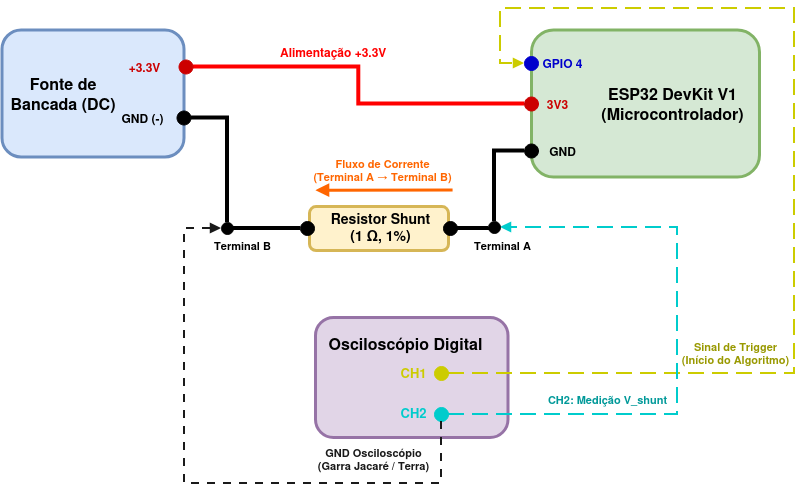
\includegraphics[scale=0.5]{figuras/setup_consumo_energia.png}
  \end{center}
  \legend{Fonte: Elaborado pelos autores (2026) com base em \cite{hubble2024esp32power}}
\end{figure}


% Capítulo 4. Especificação de Requisitos
\chapter{Especificação de Requisitos} \label{cap:especificacao}

%%%%%%%%%%%%%%%%%%%%%%%%%%%%%%%%%%%%%%%%%%%%%%%%%%%%
%%%%%%%%%%%%%%%%%%%%%%%%%%%%%%%%%%%%%%%%%%%%%%%%%%%%

\section{Especificação da arquitetura do sistema}
\label{sec:requisitos_infra}

A arquitetura especificada neste trabalho define a organização técnica da solução proposta para comunicação, encaminhamento e persistência dos dados produzidos na rede de campo. Sua função é estruturar, de forma coerente, os componentes responsáveis pela coleta das informações, pela transição entre a comunicação embarcada e a infraestrutura de aplicação, e pelo armazenamento dos dados necessários ao funcionamento do sistema e às etapas posteriores de segurança e análise.

A solução foi organizada em quatro blocos principais: nós sensores e atuadores, gateway, backend/API e persistência. No trecho de campo, os nós realizam a coleta dos dados do ambiente e transmitem mensagens curtas por meio da arquitetura LoRaWAN, atendendo aos requisitos de operação em dispositivos com restrição energética e comunicação de baixo consumo. O gateway atua como elemento intermediário entre essa rede e a infraestrutura de aplicação, concentrando as funções de recepção, registro de metadados e encaminhamento das mensagens ao backend, em conformidade com os requisitos RF3 e RF6.

A partir do gateway, a comunicação passa a utilizar Wi-Fi e requisições HTTP, permitindo integrar a rede embarcada a uma API autenticada implantada em infraestrutura de nuvem e a um mecanismo centralizado de persistência. Essa organização busca manter a camada de aplicação disponível de forma contínua para o recebimento dos dados encaminhados pelo gateway, ao mesmo tempo em que facilita o armazenamento e a posterior utilização das informações coletadas.

Além dos dados de aplicação, como temperatura e luminosidade, a arquitetura prevê a persistência de metadados relevantes para o acompanhamento da comunicação, incluindo informações de origem, sequência, recepção e qualidade do enlace. Essa escolha atende aos requisitos RF5 e RF7, além de contribuir para a rastreabilidade da operação, conforme estabelecido em RNF6. A mesma base persistida também prepara a infraestrutura para a incorporação posterior de mecanismos de criptografia leve e de análise por aprendizado de máquina, em conformidade com RNF7 e RNF8.

A Figura~\ref{fig:arquitetura-especificada} apresenta a arquitetura técnica especificada para o sistema. A partir dessa organização, as subseções seguintes detalham os requisitos funcionais e não funcionais da infraestrutura proposta, que fundamentam e justificam as decisões arquiteturais adotadas.

\begin{figure}[htb]
  \caption{\label{fig:arquitetura-especificada}Arquitetura especificada do sistema proposto.}
  \begin{center}
      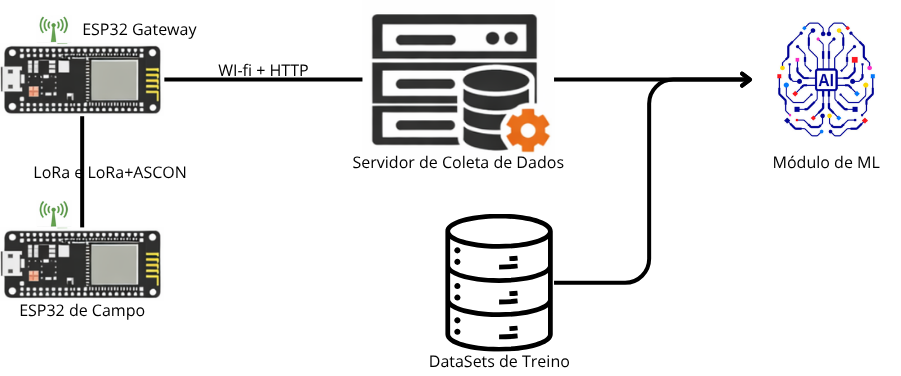
\includegraphics[scale=0.5]{figuras/arch_figure1.png}
  \end{center}

\end{figure}

%%%%%%%%%%%%%%%%%%%%%%%%%%%%%%%%%%%%%%%%%%%%%%%%%%%%

\subsection{Requisitos funcionais da infraestrutura proposta}

Os requisitos funcionais da infraestrutura proposta descrevem os comportamentos esperados da arquitetura do sistema, considerando a coleta, o encaminhamento, a autenticação e a persistência das informações produzidas na rede de campo.

\begin{enumerate}
    \item[RF1.] O sistema deve permitir que os nós de campo coletem e transmitam dados de aplicação, incluindo, no protótipo previsto, informações de temperatura e luminosidade.

    \item[RF2.] Cada mensagem transmitida pelos nós deve conter, além dos dados de aplicação, informações mínimas de identificação e acompanhamento, incluindo identificador do dispositivo e contador de mensagens.

    \item[RF3.] O gateway deve receber as mensagens provenientes da rede de campo, registrar os metadados de recepção e encaminhar essas informações ao backend por meio de rede Wi-Fi e requisições HTTP.

    \item[RF4.] O backend deve autenticar as requisições enviadas pelo gateway, restringindo o recebimento de dados a dispositivos previamente autorizados.

    \item[RF5.] O sistema deve persistir os dados de aplicação recebidos dos nós juntamente com os metadados associados à comunicação.

    \item[RF6.] A infraestrutura deve permitir armazenamento temporário das mensagens no gateway em situações de indisponibilidade da conexão com o backend, com possibilidade de reenvio posterior.

    \item[RF7.] Os dados persistidos devem permanecer disponíveis para uso posterior pelas camadas de segurança e de análise por aprendizado de máquina.
\end{enumerate}

%%%%%%%%%%%%%%%%%%%%%%%%%%%%%%%%%%%%%%%%%%%%%%%%%%%%

\subsection{Requisitos não funcionais da infraestrutura proposta}

Os requisitos não funcionais da infraestrutura proposta descrevem propriedades de operação e restrições que devem ser observadas para que a solução seja compatível com o contexto de sistemas embarcados e Internet das Coisas. Para sua elicitação e organização, adotou-se como referência a norma ISO/IEC 25010, considerando principalmente características relacionadas à eficiência de desempenho, confiabilidade, compatibilidade, manutenibilidade e segurança.

\begin{enumerate}
    \item[RNF1.] A infraestrutura deve ser compatível com a operação de nós de campo com restrições de energia, priorizando baixo consumo no trecho embarcado da comunicação.

    \item[RNF2.] A comunicação do sistema deve ser orientada a evento, evitando transmissões contínuas desnecessárias entre os componentes.

    \item[RNF3.] A arquitetura deve manter separação clara entre a rede de campo, baseada em LoRaWAN, e a infraestrutura de aplicação, baseada em Wi-Fi e HTTP.

    \item[RNF4.] O protótipo deve preservar simplicidade de integração entre hardware, comunicação e backend, de modo a manter viável sua montagem e evolução no contexto do projeto.

    \item[RNF5.] A infraestrutura deve apresentar robustez básica a falhas temporárias de conectividade entre gateway e backend.

    \item[RNF6.] O sistema deve garantir rastreabilidade das mensagens recebidas, por meio do registro de dados e metadados que permitam identificar origem, sequência, instante de recepção e condições básicas do enlace.

    \item[RNF7.] A arquitetura deve ser compatível com a incorporação posterior de mecanismos de criptografia leve sem exigir reformulação completa da infraestrutura de comunicação.

    \item[RNF8.] A infraestrutura deve ser compatível com o uso posterior de técnicas de aprendizado de máquina aplicadas à análise do comportamento da rede e à detecção de anomalias.
\end{enumerate}

%%%%%%%%%%%%%%%%%%%%%%%%%%%%%%%%%%%%%%%%%%%%%%%%%%%%
%%%%%%%%%%%%%%%%%%%%%%%%%%%%%%%%%%%%%%%%%%%%%%%%%%%%

\section{Requisitos do Sistema de Detecção de Anomalias}
A incorporação de um modelo de aprendizado de máquina à arquitetura proposta 
introduz requisitos específicos, distintos dos requisitos de infraestrutura 
definidos na Seção~\ref{sec:requisitos_infra}. O modelo será treinado e 
avaliado em ambiente computacional convencional, utilizando os dados 
históricos do \textit{dataset} Tour Perret. A viabilidade de portabilidade 
da fase de inferência para o gateway é tratada como perspectiva de 
continuidade, conforme discutido na Seção~7.3.

%%%%%%%%%%%%%%%%%%%%%%%%%%%%%%%%%%%%%%%%%%%%%%%%%%%%

\subsection{Requisitos Funcionais}

\begin{enumerate}

    \item[RF1.] O sistema deve receber como entrada sequências temporais das 
    variáveis selecionadas, organizadas por dispositivo e ordenadas 
    cronologicamente.

    \item[RF2.] O sistema deve produzir previsões do comportamento esperado de 
    cada variável monitorada e calcular o resíduo entre valor previsto e 
    valor observado para cada instante de tempo.

    \item[RF3.] O sistema deve classificar cada observação como normal ou 
    potencialmente anômala, com base em um critério de limiarização definido 
    a partir do conjunto de validação.

    \item[RF4.] O sistema deve permitir comparação quantitativa entre as três 
    abordagens de modelagem (ARIMA, RNN, LSTM) através de métricas 
    padronizadas de qualidade de previsão e detecção.

\end{enumerate}


%%%%%%%%%%%%%%%%%%%%%%%%%%%%%%%%%%%%%%%%%%%%%%%%%%%%

\subsection{Requisitos Não Funcionais}

\begin{enumerate}

    \item[RNF1.] O treinamento deve ser realizado exclusivamente sobre dados que 
    representem operação normal da rede, sem contaminação por observações 
    potencialmente anômalas.

    \item[RNF2.] O processo de treinamento e avaliação deve ser reprodutível, com 
    registro das sementes de inicialização, hiperparâmetros e critérios de 
    seleção de ordem utilizados em cada modelo.

\end{enumerate}

Essa orientação fortalece a coerência do trabalho como um todo. Em vez de separar artificialmente a fase de modelagem da fase de implantação, o desenvolvimento já considera que a utilidade prática dos modelos depende de um equilíbrio entre eficácia de detecção e viabilidade de execução em dispositivos restritos. Assim, a implementação proposta dialoga diretamente com a etapa posterior de avaliação energética e computacional.

Sob essa perspectiva, a comparação entre modelos não deverá considerar apenas métricas tradicionais de desempenho, mas também aspectos como simplicidade estrutural, custo computacional, volume de memória.

%%%%%%%%%%%%%%%%%%%%%%%%%%%%%%%%%%%%%%%%%%%%%%%%%%%%
%%%%%%%%%%%%%%%%%%%%%%%%%%%%%%%%%%%%%%%%%%%%%%%%%%%%

\section{Requisitos de Segurança do Sistema criptográfico}
\subsection{Segurança do Ascon-AEAD128}
Para o uso seguro da cifra, este trabalho adota os requisitos operacionais especificados pelo NIST para o Ascon-AEAD128 \cite{nist800232}. Embora a implementação utilizada corresponda à variante Ascon-128a (versão 1.2), esses requisitos são adotados de forma conservadora como limites aplicáveis, uma vez que ambas as versões compartilham a mesma taxa de processamento e a mesma estrutura de permutação, enquanto suas diferenças introduzem apenas sobrecarga constante. O primeiro requisito trata da geração da chave criptográfica, que deve seguir os padrões descritos no documento SP 800-133r2 \citeonline{barker2020nist133}, no qual é estabelecida a seguinte operação:

\[
K = U \oplus V,
\]

em que $U$ é uma cadeia de bits extraída de um Gerador de Bits Aleatórios (RBG - \textit{Random Bit Generator}) aprovado, e $V$ consiste em uma sequência de bits gerada independentemente de $U$, podendo ser composta inteiramente por zeros.

As especificações para os geradores de bits aleatórios aprovados estão descritas no documento SP 800-90A \citeonline{barker2015nist90a}. Neste projeto, será utilizado um Gerador Determinístico de Bits Aleatórios (DRBG - \textit{Deterministic Random Bit Generator}) através do mecanismo CTR\_DRBG. Essa escolha justifica-se pelo fato de que a entropia bruta extraída diretamente do hardware pode conter vícios físicos, tornando indispensável um estágio secundário de tratamento e condicionamento algorítmico \cite{turan2018nist90b}. Dessa forma, a implementação fará uso da biblioteca nativa \textit{mbedTLS} do ESP32, que extrai a entropia verdadeira do periférico de hardware (TRNG) e a processa através do algoritmo CTR\_DRBG, garantindo uma saída perfeitamente balanceada para a geração da chave.

Com base nesses elementos, os requisitos de segurança do Ascon-AEAD128 podem ser organizados em requisitos funcionais e não funcionais.

\subsubsection{Requisitos funcionais}

\begin{enumerate}
    \item[RF1.] A implementação da biblioteca \textit{ascon-suite} deve ser validada previamente, conforme discutido na Seção \ref{subsec:validacao-ascon}.

    \item[RF2.] A geração da chave criptográfica deve seguir os padrões descritos no documento SP 800-133r2 \citeonline{barker2020nist133}, adotando a operação $K = U \oplus V$.

    \item[RF3.] O sistema deve utilizar um Gerador Determinístico de Bits Aleatórios (DRBG - \textit{Deterministic Random Bit Generator}) através do mecanismo CTR\_DRBG para a geração de chaves criptográficas.

    \item[RF4.] A implementação deve fazer uso da biblioteca nativa \textit{mbedTLS} do ESP32 para extrair a entropia verdadeira do periférico de hardware (TRNG) e processá-la através do algoritmo CTR\_DRBG.

    \item[RF5.] Caso a renovação da chave simétrica se faça necessária por eventuais comprometimentos ou políticas de segurança, o sistema deve adotar o método de encapsulamento de chaves (\textit{key wrapping}), utilizando a chave secreta atual, desde que ainda válida e segura, para cifrar a nova chave gerada e permitir seu compartilhamento e atualização de forma segura entre o dispositivo e o nó de borda (\textit{Edge}).
\end{enumerate}

\subsubsection{Requisitos não funcionais}

\begin{enumerate}
    \item[RNF1.] A entropia bruta extraída diretamente do hardware não deve ser utilizada sem tratamento adicional, uma vez que pode conter vícios físicos (\textit{bias}), tornando indispensável um estágio secundário de condicionamento algorítmico \cite{turan2018nist90b}.

    \item[RNF2.] A chave criptográfica deve ser mantida em sigilo absoluto, aliada à garantia de unicidade do \textit{nonce} para cada operação de encriptação.

    \item[RNF3.] Para \textit{tags} de autenticação cujo tamanho $\lambda$ (em bits) satisfaça a condição $64 \leq \lambda \leq 128$, a quantidade de falhas de decriptação não deve exceder $2^{\lambda - 32}$.

    \item[RNF4.] O volume máximo de dados processados durante as rotinas de encriptação e decriptação não deve ultrapassar $2^{54}$ bytes para uma mesma chave, devendo a chave ser obrigatoriamente renovada caso esse limite seja atingido.
\end{enumerate}

Diante desses requisitos, alguns deles possuem impacto prático reduzido no contexto deste projeto. Como as redes LoRaWAN operam com taxas de transmissão extremamente baixas e pacotes pequenos, atingir o limite de $2^{54}$ bytes processados sob uma mesma chave é inviável durante a vida útil física do dispositivo. Da mesma forma, considerando o uso de uma \textit{tag} de 128 bits, o limite tolerado antes da obrigatoriedade de rotação da chave é de $2^{96}$ falhas de decriptação. Alcançar esse volume de tentativas de ataques de injeção na rede é improvável, dadas as severas restrições de tempo de transmissão inerentes ao protocolo.


% Capítulo 5. Desenvolvimento
\chapter{Desenvolvimento do Trabalho} \label{cap:desenvolvimento}
\section{Atividades Previstas}

\subsection{Implementação da infraestrutura}

A implementação da infraestrutura corresponde à etapa inicial de desenvolvimento da solução proposta. Nessa fase, o objetivo é estabelecer a base de comunicação e persistência do sistema, permitindo integrar os nós de campo, o gateway e a camada de backend antes da incorporação dos mecanismos de segurança e análise.

Inicialmente, a implementação deverá concentrar-se na comunicação entre os dispositivos de campo e o gateway, utilizando placas com suporte integrado a LoRa. Os nós serão responsáveis pela coleta dos dados de aplicação e pela transmissão de mensagens curtas, enquanto o gateway atuará como ponto de recepção e transição entre a rede de campo e a infraestrutura de aplicação.

Após a recepção das mensagens, o gateway deverá organizar os dados recebidos, registrar metadados associados à comunicação e encaminhar essas informações ao backend por meio de conectividade Wi-Fi e requisições HTTP. No backend, será implementada uma API com mecanismo de autenticação, de modo a restringir o recebimento de dados a gateways autorizados.

Além do encaminhamento das mensagens, essa etapa também deverá contemplar a persistência dos dados de aplicação e dos metadados de comunicação em banco de dados. Esse armazenamento é necessário para o acompanhamento do funcionamento do sistema e para dar suporte às etapas posteriores do trabalho, especialmente aquelas relacionadas à segurança e à análise do comportamento da rede.

Por fim, a implementação da infraestrutura deverá prever um mecanismo básico de robustez para falhas temporárias de conectividade entre gateway e backend. Para isso, admite-se o uso de armazenamento local temporário no gateway, com reenvio posterior das mensagens quando a conexão for restabelecida. Com essa etapa, estabelece-se a base operacional mínima da solução, sobre a qual serão incorporadas, posteriormente, as camadas de criptografia leve e de aprendizado de máquina.


%%%%%%%%%%%%%%%%%%%%%%%%%%%%%%%%%%%%%%%%%%%%%%%%%%%%


\subsection{Segurança com Ascon}
Para o desenvolvimento da camada de segurança com o padrão Ascon, o trabalho seguirá um roteiro de atividades práticas de implementação, validação e coleta de dados diretamente no hardware. As atividades previstas para essa frente de trabalho são:

\begin{itemize}
    \item \textbf{Integração da biblioteca:} Instalar e configurar a biblioteca \textit{ascon-suite} no ambiente do ESP32, criando o código necessário para conectar a criptografia com o envio de pacotes LoRaWAN.
    
    \item \textbf{Validação Matemática (KAT):} Rodar os testes oficiais (\textit{Known Answer Tests}) no computador para garantir que a biblioteca calcula as cifras corretamente. Depois, embarcar uma parte desses testes no próprio ESP32 para confirmar que não ocorreram erros durante a compilação para o microcontrolador.
    
    \item \textbf{Geração de Chaves:} Escrever o código para gerar as chaves criptográficas. Para isso, será usado o gerador de números aleatórios do hardware do ESP32 (TRNG) em conjunto com a função \textit{CTR\_DRBG} da biblioteca \textit{mbedTLS}, seguindo as recomendações oficiais do NIST.
    
    \item \textbf{Testes de Injeção de Falhas:} Criar um código de estresse que altere os pacotes de propósito (\textit{bit-flipping}). A ideia é corromper o texto cifrado, o cabeçalho LoRaWAN e a \textit{tag} de autenticação para provar que a função de descriptografia bloqueia a mensagem imediatamente.
    
    \item \textbf{Coleta de Métricas (Benchmarking):} Realizar as medições práticas de desempenho. Isso inclui contar os ciclos de \textit{clock} para o tempo de execução, monitorar os picos de memória (Heap e Stack) e medir o consumo de energia com o osciloscópio e o resistor \textit{shunt}.
\end{itemize}

%%%%%%%%%%%%%%%%%%%%%%%%%%%%%%%%%%%%%%%%%%%%%%%%%%%%

\subsection{Modelo de Machine Learning}

O desenvolvimento da frente de aprendizado de máquina seguirá um conjunto de
atividades voltadas à preparação dos dados, treinamento dos modelos e avaliação
da capacidade de detecção de anomalias. O objetivo dessa etapa é construir uma
base experimental consistente para comparar diferentes abordagens de regressão
temporal aplicadas ao comportamento da rede LoRaWAN.

As atividades previstas para essa frente de trabalho são:
\begin{itemize}
    \item \textbf{Preparação dos datasets:} Organizar os dados selecionados para a etapa de modelagem, com foco principal no dataset Tour Perret e uso complementar do dataset GUARD. Essa preparação incluirá harmonização de timestamps, tratamento de valores ausentes, extração dos atributos relevantes e organização das observações por dispositivo.

    \item \textbf{Definição e seleção de variáveis:} Avaliar os atributos disponíveis nos datasets e selecionar o subconjunto de variáveis mais adequado para a modelagem temporal do comportamento normal da rede. Entre os candidatos principais estão RSSI, SNR, FCnt, \textit{inter-arrival time} e \textit{data rate}, considerando sua estabilidade temporal, disponibilidade e relevância para a identificação de desvios.

    \item \textbf{Divisão temporal dos dados:} Separar os dados em conjuntos de treinamento (60\%), validação (20\%) e teste (20\%) por meio de uma divisão cronológica, preservando a ordem temporal das observações e evitando vazamento de informação futura para o treinamento dos modelos.

    \item \textbf{Exploração e seleção de arquiteturas:} Implementar os modelos ARIMA, RNN e LSTM definidos na etapa metodológica do trabalho. Para cada modelo, será realizada uma exploração de hiperparâmetros e configurações arquiteturais com o objetivo de identificar combinações adequadas ao problema. A seleção de configurações será orientada por critérios de desempenho preditivo e simplicidade estrutural, priorizando modelos com menor complexidade quando o ganho de performance for marginal.

    \item \textbf{Treinamento exclusivo em dados normais:} Todos os modelos serão treinados e validados exclusivamente com dados representativos da operação normal da rede (dataset Tour Perret), garantindo que o comportamento esperado seja aprendido sem contaminação por anomalias ou ataques.

    \item \textbf{Avaliação da qualidade preditiva:} Comparar os modelos com base em métricas de erro de regressão (MAE e RMSE) no conjunto de teste, com o objetivo de verificar qual abordagem representa com maior fidelidade o comportamento esperado das variáveis monitoradas.

    \item \textbf{Calibração de limiar de detecção:} Com base nos resíduos do conjunto de validação, será definido um critério de limiarização (baseado em desvio padrão ou percentis) para classificar observações como normais ou potencialmente anômalas.

    \item \textbf{Avaliação da capacidade de detecção:} Analisar a performance de detecção dos modelos no conjunto de teste e também na aplicação aos dados do dataset GUARD, com o objetivo de verificar se os modelos conseguem identificar anomalias quando confrontados com padrões diferentes ou com ataques conhecidos. Será utilizada a métrica de teste de generalização para avaliar robustez.

    \item \textbf{Análise de viabilidade para execução em borda:} Após a comparação entre os modelos, será realizada uma análise complementar da complexidade das soluções obtidas, considerando número de parâmetros, custo computacional e compatibilidade com uma eventual etapa futura de adaptação para TinyML.
\end{itemize}

%%%%%%%%%%%%%%%%%%%%%%%%%%%%%%%%%%%%%%%%%%%%%%%%%%%%

\subsection{Integração progressiva da solução}

A implementação proposta neste trabalho foi organizada de forma progressiva, de modo que cada etapa estabeleça a base necessária para a etapa seguinte. Inicialmente, a prioridade está na consolidação da infraestrutura de comunicação e persistência, garantindo que os dados produzidos em campo possam ser recebidos, encaminhados, autenticados e armazenados de forma consistente.

Sobre essa base, será incorporada a camada de segurança com o uso do padrão Ascon, com foco na proteção do payload gerado pelos nós de campo. Essa etapa permitirá avaliar a inserção dos mecanismos criptográficos sem alterar a organização principal da infraestrutura já estabelecida, preservando a separação entre comunicação, autenticação e persistência.

Em seguida, a base de dados formada pela operação da infraestrutura será utilizada na etapa de análise por aprendizado de máquina. Nessa fase, tanto os dados de aplicação quanto os metadados de comunicação poderão ser explorados com o objetivo de apoiar a análise do comportamento da rede e a identificação de padrões associados a anomalias.

Dessa forma, a proposta não trata infraestrutura, segurança e análise como frentes independentes, mas como partes complementares de uma mesma solução. A integração progressiva dessas camadas permite desenvolver o sistema com maior clareza, reduz a complexidade da implementação inicial e favorece a avaliação da arquitetura como um todo.

%%%%%%%%%%%%%%%%%%%%%%%%%%%%%%%%%%%%%%%%%%%%%%%%%%%%%%
%%%%%%%%%%%%%%%%%%%%%%%%%%%%%%%%%%%%%%%%%%%%%%%%%%%%%%

\section{Resultados dos Testes da Camada de Segurança (Ascon)}

Esta seção reúne os resultados dos testes de validação e avaliação da camada de segurança baseada no Ascon, seguindo a metodologia definida na Seção \ref{subsec:validacao-ascon}. Os resultados são incorporados de forma progressiva, à medida que cada etapa de teste é concluída.

%%%%%%%%%%%%%%%%%%%%%%%%%%%%%%%%%%%%%%%%%%%%%%%%%%%%%%

\subsection{Validação por \textit{Known Answer Tests} (KAT)}

A validação funcional foi conduzida com os vetores oficiais do Ascon-128a (versão 1.2) distribuídos com a \textit{ascon-suite}. Inicialmente, a biblioteca foi compilada em um computador \textit{desktop} e submetida à execução exaustiva dos 1089 vetores de teste, nos quais cada combinação de chave, \textit{nonce}, dados associados e texto em claro deve produzir um texto cifrado e uma \textit{tag} de autenticação exatos.

Todos os 1089 vetores foram processados com correspondência integral em relação às saídas esperadas, sem nenhuma falha. Como verificação adicional, os vetores foram regenerados a partir da própria implementação e comparados byte a byte com o arquivo de referência, resultando em arquivos idênticos. Por fim, a suíte de testes automatizados (\textit{CTest}) foi executada sobre as variantes em C, C++, \textit{SIV} e mascarada do algoritmo, com aprovação nos 14 casos avaliados. A Tabela~\ref{tab:kat_ascon128a} sintetiza esses resultados.

\begin{table}[htb]
\centering
\caption{Resultado da validação por \textit{Known Answer Tests} do Ascon-128a}
\label{tab:kat_ascon128a}
\begin{tabular}{lrr}
\hline
\textbf{Verificação} & \textbf{Casos} & \textbf{Falhas} \\
\hline
Execução exaustiva (\textit{desktop})                  & 1089 vetores & 0 \\
Regeneração \textit{vs.} referência                    & 1089 vetores & 0 \\
Suíte \textit{CTest} (C, C++, \textit{SIV}, mascarada) & 14 testes    & 0 \\
Execução na placa (ESP32, subconjunto)                 & 6 vetores    & 0 \\
\hline
\end{tabular}
\legend{Fonte: elaborado pelos autores.}
\end{table}

Esses resultados comprovam que a implementação do Ascon-128a opera corretamente no ambiente de desenvolvimento, reproduzindo de forma exata os valores de referência do algoritmo.

Confirmada a correção em \textit{desktop}, um subconjunto representativo dos vetores foi executado diretamente na placa ESP32, cobrindo os limites de processamento por blocos: entrada vazia, bloco parcial, bloco completo e múltiplos blocos, com e sem dados associados. Para cada vetor, verificaram-se tanto a cifração — comparando o resultado com o valor de referência — quanto a decifração, confirmando a recuperação do texto claro com a \textit{tag} validada. Os seis vetores foram reproduzidos com correspondência integral na placa, descartando divergências introduzidas pela compilação ou pela arquitetura do \textit{hardware} (Xtensa LX, \textit{little-endian}). Nessa execução, o estado interno do algoritmo (\texttt{ascon128a\_state\_t}) ocupou 80 bytes, valor retomado posteriormente na análise de memória.

Os vetores utilizados e o registro completo das execuções, em \textit{desktop} e na placa, estão disponíveis no repositório do projeto, na pasta \texttt{kat-validation}.

%%%%%%%%%%%%%%%%%%%%%%%%%%%%%%%%%%%%%%%%%%%%%%%%%%%%%%

\subsection{Validação dos Dados Associados (AEAD)}

A propriedade de autenticação do modo AEAD foi avaliada na placa ESP32 por injeção intencional de falhas (\textit{bit-flipping}), simulando um ataque de \textit{Man-in-the-middle}. A partir de um pacote válido (texto claro de 28 bytes e dados associados de 26 bytes), cada bit das três frentes de adulteração — texto cifrado, dados associados e \textit{tag} de autenticação — foi invertido individualmente, e a mensagem resultante foi submetida à decifragem.

Como controle, o pacote intacto foi decifrado com sucesso, recuperando o texto claro original. Já as 560 adulterações de um bit foram todas rejeitadas: a função de decifragem reconheceu a quebra de integridade e falhou imediatamente, sem entregar qualquer fragmento de texto claro. A Tabela~\ref{tab:aead_ascon128a} resume os resultados.

\begin{table}[htb]
\centering
\caption{Rejeição de adulterações (\textit{bit-flipping}) no Ascon-128a}
\label{tab:aead_ascon128a}
\begin{tabular}{lrr}
\hline
\textbf{Frente de adulteração} & \textbf{Bits testados} & \textbf{Rejeições} \\
\hline
Texto cifrado (\textit{ciphertext}) & 224 & 224 \\
Dados associados (AD)               & 208 & 208 \\
\textit{Tag} de autenticação        & 128 & 128 \\
\hline
Total                               & 560 & 560 \\
\hline
\end{tabular}
\legend{Fonte: elaborado pelos autores.}
\end{table}

Qualquer modificação na mensagem em trânsito — no \textit{payload}, nos metadados do cabeçalho ou na própria \textit{tag} — é detectada e rejeitada, garantindo a integridade e a autenticidade contra ataques de \textit{Man-in-the-middle}. O código de teste está no repositório, na pasta \texttt{aead-validation}.

%%%%%%%%%%%%%%%%%%%%%%%%%%%%%%%%%%%%%%%%%%%%%%%%%%%%%%

\subsection{Consumo de Memória e Tempo de Execução}

O custo de memória e de tempo do Ascon-128a foi medido diretamente na placa ESP32, a 240~MHz. Quanto à memória, a operação de cifragem não realiza nenhuma alocação dinâmica: o \textit{heap} livre permaneceu inalterado antes e depois da execução (delta de 0 bytes) e o estado interno do algoritmo (\texttt{ascon128a\_state\_t}) ocupa apenas 80 bytes. Em relação à memória de programa (\textit{Flash}), a inclusão da biblioteca acrescentou 7.048 bytes ao \textit{firmware} (294.352 bytes com a biblioteca contra 287.304 bytes sem ela), o equivalente a cerca de 6,9~KiB, ou 0,5\% da \textit{Flash} disponível.

O tempo de execução foi obtido lendo o contador de ciclos da CPU, com as interrupções desabilitadas durante cada medição para eliminar o ruído de tratadores de interrupção. A Tabela~\ref{tab:tempo_ascon128a} apresenta o custo de cifragem para diferentes tamanhos de \textit{payload}. O tempo cresce de forma aproximadamente linear com o número de blocos de 128 bits, sobre uma base fixa de inicialização e finalização: cada bloco adicional acrescenta cerca de 1.100 ciclos.

\begin{table}[htb]
\centering
\caption{Tempo de cifragem do Ascon-128a no ESP32 (240~MHz)}
\label{tab:tempo_ascon128a}
\begin{tabular}{rrr}
\hline
\textbf{Payload} & \textbf{Ciclos} & \textbf{Tempo ($\mu$s)} \\
\hline
16 bytes & 6.117 & 25,49 \\
32 bytes & 7.214 & 30,06 \\
64 bytes & 9.408 & 39,20 \\
\hline
\end{tabular}
\legend{Fonte: elaborado pelos autores.}
\end{table}

Por fim, avaliou-se a resistência a ataques de canal colateral baseados em tempo. Ao executar 5.000 cifragens de 16 bytes com chaves e conteúdos distintos, porém de tamanho fixo, a variação relativa do número de ciclos foi de apenas 0,005\% (desvio padrão sobre a média) e o valor mínimo permaneceu invariante (6.117 ciclos), independentemente do conteúdo. Esse comportamento corrobora a propriedade de tempo constante do Ascon — decorrente de seu projeto sem ramificações ou acessos a tabelas dependentes de dados —, impedindo que um atacante infira fragmentos da chave ou da mensagem a partir do tempo de processamento do nó sensor.

%%%%%%%%%%%%%%%%%%%%%%%%%%%%%%%%%%%%%%%%%%%%%%%%%%%%%%

\subsection{Comparativo com AES-128-GCM}

Para responder à questão central levantada na Seção 2.2.2 — se a migração para criptografia leve em software traz vantagem real frente ao acelerador de \textit{hardware} já presente nas placas comerciais —, comparou-se o Ascon-128a (software) com o AES-128-GCM (\textit{Galois/Counter Mode}) na mesma execução e sob as mesmas condições (ESP32 a 240~MHz). O AES-GCM foi avaliado por meio da biblioteca \textit{mbedTLS} do próprio \textit{core} do ESP32. Cabe ressaltar que, no ESP32 clássico, apenas o bloco AES é executado no acelerador de \textit{hardware}; a autenticação (GHASH) permanece em software, pois o GCM inteiramente em hardware só está disponível em variantes mais recentes (S2/S3/C3).

Quanto à memória, ambos os algoritmos operaram sem qualquer alocação dinâmica (variação de \textit{heap} nula). Quanto ao tempo, mediu-se a latência de cifragem pelo número mínimo de ciclos de \textit{clock} (piso livre de interrupções) ao longo de 2.000 execuções. A Tabela~\ref{tab:comparativo_aes} apresenta os resultados.

\begin{table}[htb]
\centering
\caption{Latência de cifragem: Ascon-128a (software) \textit{vs.} AES-128-GCM (hardware) no ESP32}
\label{tab:comparativo_aes}
\begin{tabular}{rrrr}
\hline
\textbf{Payload} & \textbf{Ascon-128a} & \textbf{AES-128-GCM} & \textbf{Razão} \\
                 & \textbf{ciclos ($\mu$s)} & \textbf{ciclos ($\mu$s)} & \textbf{AES/Ascon} \\
\hline
16 bytes & 6.115 (25,5) & 8.541 (35,6)  & 1,40 \\
32 bytes & 7.212 (30,1) & 10.650 (44,4) & 1,48 \\
64 bytes & 9.406 (39,2) & 14.868 (62,0) & 1,58 \\
\hline
\end{tabular}
\legend{Fonte: elaborado pelos autores.}
\end{table}

Em todos os tamanhos avaliados, o Ascon-128a em software foi mais rápido que o AES-128-GCM acelerado por \textit{hardware}, com vantagem entre 1,40 e 1,58 vez. Decompondo o custo, cada bloco de 128 bits acrescenta cerca de 1.097 ciclos no Ascon contra 2.109 ciclos no AES-GCM — aproximadamente o dobro. Esse custo por bloco mais elevado decorre do GHASH executado em software e explica por que a vantagem do Ascon aumenta com o tamanho do \textit{payload}. Para os pacotes pequenos típicos de redes LoRaWAN, portanto, a criptografia leve em software não apenas dispensa o acelerador de \textit{hardware} como o supera em latência, mantendo ainda a ausência de alocação dinâmica de memória.

Ressalva-se que esse resultado se refere ao ESP32 clássico; em microcontroladores com suporte a GCM inteiramente em \textit{hardware}, a comparação poderia favorecer o AES-GCM. A avaliação de consumo energético dessa mesma comparação, descrita na Seção 3.4.4, complementará esta análise.


% Capítulo 6. Considerações
\chapter{Considerações Preliminares} \label{cap:consideracoes}

Até a presente etapa de desenvolvimento do trabalho, os esforços foram concentrados na consolidação da fundamentação teórica, na revisão bibliográfica e na especificação da arquitetura do sistema. O trabalho estabeleceu a base conceitual necessária para a integração segura de dispositivos IoT em redes LoRaWAN, definindo os papéis do nó sensor, do \textit{gateway} e da infraestrutura de \textit{backend}. 

Durante a fase de especificação, foi possível justificar tecnicamente as escolhas das tecnologias que comporão o protótipo. Selecionou-se a família Ascon — na variante Ascon-128a (v1.2), de mesma estrutura de permutação do Ascon-AEAD128 padronizado — para garantir confidencialidade e integridade com baixo custo computacional, superando alternativas legadas em ambientes restritos. Em paralelo, a estratégia de aprendizado de máquina foi definida, optando-se por modelos de regressão temporal não supervisionados (utilizando os \textit{datasets} Tour Perret e GUARD) como mecanismo de detecção de anomalias operacionais.

\section{Perspectivas de Continuidade}

O presente trabalho estabelece uma arquitetura de segurança integrada para 
redes LoRaWAN, combinando criptografia leve por meio do padrão Ascon e 
detecção de anomalias via modelos de regressão temporal. Embora os objetivos 
definidos para este projeto sejam tratados de forma completa nas etapas 
descritas nos capítulos anteriores, a natureza do problema abre caminhos 
relevantes para investigações futuras.

A perspectiva de maior interesse imediato diz respeito à portabilidade da 
fase de inferência dos modelos treinados para o próprio gateway da rede. 
Neste trabalho, o treinamento e a avaliação dos modelos são realizados em 
ambiente computacional convencional, decisão justificada pelas restrições de 
hardware incompatíveis com o processo de treinamento. Contudo, uma vez 
obtido um modelo com desempenho satisfatório, torna-se pertinente investigar 
se sua fase de inferência pode ser executada diretamente no gateway, 
eliminando a necessidade de transmissão dos dados brutos para uma camada 
externa de processamento.

Essa investigação demandaria a análise da complexidade do modelo resultante 
— em termos de número de parâmetros, tamanho serializado e tempo de 
inferência — em relação às restrições de memória RAM e armazenamento em 
\textit{flash} do hardware adotado. Ferramentas como o TensorFlow Lite for 
Microcontrollers e a biblioteca \textit{emlearn} permitem a conversão de 
modelos treinados em Python para código C otimizado, compatível com 
microcontroladores como o ESP32 \cite{ray2022}. Técnicas de compressão como 
quantização de pesos e poda de conexões poderiam ser aplicadas para reduzir 
o custo computacional sem perda significativa de desempenho \cite{jacob2018}.

Uma segunda perspectiva relevante envolve a extensão da abordagem de 
detecção para incorporar dados rotulados de ataque, como os disponíveis no 
\textit{dataset} GUARD. Com resultados de regressão consolidados sobre o 
Tour Perret, seria possível investigar em que medida os resíduos produzidos 
pelos modelos se comportam de forma diferenciada diante de \textit{frames} 
reconhecidamente manipulados, abrindo caminho para uma avaliação mais 
rigorosa da capacidade de detecção em cenários com ataques conhecidos.

Por fim, a arquitetura proposta poderia ser estendida para contemplar 
mecanismos de atualização contínua do modelo, permitindo que o sistema se 
adapte a mudanças graduais no comportamento da rede — como variações 
sazonais de sinal ou substituição de dispositivos — sem comprometer a 
sensibilidade à detecção de anomalias. Essa capacidade de adaptação é 
especialmente relevante em implantações de longa duração, características 
de aplicações industriais e de cidades inteligentes.

%%%%%%%%%%%%%%%%%%%%%%%%%%%%%%%%%%%%%%%%%%%%%%%%%%%%

\subsection{Segurança Física do ESP32}
A implementação Ascon-128a fornece confidencialidade e integridade para os dados em trânsito, mas a integridade do sistema como um todo depende do sigilo da chave criptográfica armazenada no nó sensor. Como dispositivos de borda (\textit{Edge}) operam em ambientes fisicamente hostis e não supervisionados, são alvos potenciais para ataques de extração de memória (\textit{Flash Dumping}).

O escopo desta pesquisa concentrou-se na eficiência das primitivas criptográficas; para uma implantação real, porém, a segurança em nível de hardware é uma camada indispensável.

Para mitigar essas vulnerabilidades físicas em desenvolvimentos futuros, recomenda-se a adoção dos mecanismos nativos de segurança da família ESP32 \cite{espressif2024flash} \cite{kosemen2021tamper}. A chave simétrica do Ascon pode ser protegida com \textit{Flash Encryption} sobre a partição não-volátil (NVS), com a chave mestre gravada nos \textit{eFuses} (OTP) e protegida contra leitura externa (\textit{Read Protect}); a Inicialização Segura (\textit{Secure Boot}), que verifica a assinatura do \textit{firmware} a cada inicialização, previne regravação maliciosa. Assim, a eficiência criptográfica do Ascon opera sobre uma base de hardware que protege os dados em repouso e o código contra acesso físico não autorizado.

% ---
% Capitulo com exemplos de comandos inseridos de arquivo externo 
% ---
% \include{abntex2-modelo-include-comandos}
% ---
% Conteúdos específicos do modelo de trabalho acadêmico
% \include{quadros}

% ----------------------------------------------------------
% Finaliza a parte no bookmark do PDF
% para que se inicie o bookmark na raiz
% e adiciona espaço de parte no Sumário
% ----------------------------------------------------------
\phantompart

% ---
% Conclusão
% ---
% Capítulo 6. Considerações Finais
% \chapter{Considerações Preliminares} \label{cap:consideracoes}

Até a presente etapa de desenvolvimento do trabalho, os esforços foram concentrados na consolidação da fundamentação teórica, na revisão bibliográfica e na especificação da arquitetura do sistema. O trabalho estabeleceu a base conceitual necessária para a integração segura de dispositivos IoT em redes LoRaWAN, definindo os papéis do nó sensor, do \textit{gateway} e da infraestrutura de \textit{backend}. 

Durante a fase de especificação, foi possível justificar tecnicamente as escolhas das tecnologias que comporão o protótipo. Selecionou-se a família Ascon — na variante Ascon-128a (v1.2), de mesma estrutura de permutação do Ascon-AEAD128 padronizado — para garantir confidencialidade e integridade com baixo custo computacional, superando alternativas legadas em ambientes restritos. Em paralelo, a estratégia de aprendizado de máquina foi definida, optando-se por modelos de regressão temporal não supervisionados (utilizando os \textit{datasets} Tour Perret e GUARD) como mecanismo de detecção de anomalias operacionais.

\section{Perspectivas de Continuidade}

O presente trabalho estabelece uma arquitetura de segurança integrada para 
redes LoRaWAN, combinando criptografia leve por meio do padrão Ascon e 
detecção de anomalias via modelos de regressão temporal. Embora os objetivos 
definidos para este projeto sejam tratados de forma completa nas etapas 
descritas nos capítulos anteriores, a natureza do problema abre caminhos 
relevantes para investigações futuras.

A perspectiva de maior interesse imediato diz respeito à portabilidade da 
fase de inferência dos modelos treinados para o próprio gateway da rede. 
Neste trabalho, o treinamento e a avaliação dos modelos são realizados em 
ambiente computacional convencional, decisão justificada pelas restrições de 
hardware incompatíveis com o processo de treinamento. Contudo, uma vez 
obtido um modelo com desempenho satisfatório, torna-se pertinente investigar 
se sua fase de inferência pode ser executada diretamente no gateway, 
eliminando a necessidade de transmissão dos dados brutos para uma camada 
externa de processamento.

Essa investigação demandaria a análise da complexidade do modelo resultante 
— em termos de número de parâmetros, tamanho serializado e tempo de 
inferência — em relação às restrições de memória RAM e armazenamento em 
\textit{flash} do hardware adotado. Ferramentas como o TensorFlow Lite for 
Microcontrollers e a biblioteca \textit{emlearn} permitem a conversão de 
modelos treinados em Python para código C otimizado, compatível com 
microcontroladores como o ESP32 \cite{ray2022}. Técnicas de compressão como 
quantização de pesos e poda de conexões poderiam ser aplicadas para reduzir 
o custo computacional sem perda significativa de desempenho \cite{jacob2018}.

Uma segunda perspectiva relevante envolve a extensão da abordagem de 
detecção para incorporar dados rotulados de ataque, como os disponíveis no 
\textit{dataset} GUARD. Com resultados de regressão consolidados sobre o 
Tour Perret, seria possível investigar em que medida os resíduos produzidos 
pelos modelos se comportam de forma diferenciada diante de \textit{frames} 
reconhecidamente manipulados, abrindo caminho para uma avaliação mais 
rigorosa da capacidade de detecção em cenários com ataques conhecidos.

Por fim, a arquitetura proposta poderia ser estendida para contemplar 
mecanismos de atualização contínua do modelo, permitindo que o sistema se 
adapte a mudanças graduais no comportamento da rede — como variações 
sazonais de sinal ou substituição de dispositivos — sem comprometer a 
sensibilidade à detecção de anomalias. Essa capacidade de adaptação é 
especialmente relevante em implantações de longa duração, características 
de aplicações industriais e de cidades inteligentes.

%%%%%%%%%%%%%%%%%%%%%%%%%%%%%%%%%%%%%%%%%%%%%%%%%%%%

\subsection{Segurança Física do ESP32}
A implementação Ascon-128a fornece confidencialidade e integridade para os dados em trânsito, mas a integridade do sistema como um todo depende do sigilo da chave criptográfica armazenada no nó sensor. Como dispositivos de borda (\textit{Edge}) operam em ambientes fisicamente hostis e não supervisionados, são alvos potenciais para ataques de extração de memória (\textit{Flash Dumping}).

O escopo desta pesquisa concentrou-se na eficiência das primitivas criptográficas; para uma implantação real, porém, a segurança em nível de hardware é uma camada indispensável.

Para mitigar essas vulnerabilidades físicas em desenvolvimentos futuros, recomenda-se a adoção dos mecanismos nativos de segurança da família ESP32 \cite{espressif2024flash} \cite{kosemen2021tamper}. A chave simétrica do Ascon pode ser protegida com \textit{Flash Encryption} sobre a partição não-volátil (NVS), com a chave mestre gravada nos \textit{eFuses} (OTP) e protegida contra leitura externa (\textit{Read Protect}); a Inicialização Segura (\textit{Secure Boot}), que verifica a assinatura do \textit{firmware} a cada inicialização, previne regravação maliciosa. Assim, a eficiência criptográfica do Ascon opera sobre uma base de hardware que protege os dados em repouso e o código contra acesso físico não autorizado.

% ----------------------------------------------------------
% ELEMENTOS PÓS-TEXTUAIS
% ----------------------------------------------------------
\postextual
% ----------------------------------------------------------

% ----------------------------------------------------------
% Referências bibliográficas
% ----------------------------------------------------------

\bibliography{abntex2-modelo-references}

% ----------------------------------------------------------
% Glossário
% ----------------------------------------------------------
%
% Consulte o manual da classe abntex2 para orientações sobre o glossário.
%
%\glossary

% ----------------------------------------------------------
% Apêndices
% ----------------------------------------------------------

% ---
% Inicia os apêndices
% ---
% \begin{apendicesenv}

% % Imprime uma página indicando o início dos apêndices
% \partapendices

% % ----------------------------------------------------------
% \chapter{Quisque libero justo}
% % ----------------------------------------------------------

% \lipsum[50]

% % ----------------------------------------------------------
% \chapter{Nullam elementum urna vel imperdiet sodales elit ipsum pharetra ligula
% ac pretium ante justo a nulla curabitur tristique arcu eu metus}
% % ----------------------------------------------------------
% \lipsum[55-57]

% \end{apendicesenv}
% % ---


% ----------------------------------------------------------
% Anexos
% ----------------------------------------------------------

% ---
% Inicia os anexos
% ---
% \begin{anexosenv}

% % Imprime uma página indicando o início dos anexos
% \partanexos

% % ---
% \chapter{Morbi ultrices rutrum lorem.}
% % ---
% \lipsum[30]

% % ---
% \chapter{Cras non urna sed feugiat cum sociis natoque penatibus et magnis dis
% parturient montes nascetur ridiculus mus}
% % ---

% \lipsum[31]

% % ---
% \chapter{Fusce facilisis lacinia dui}
% % ---

% \lipsum[32]

% \end{anexosenv}

%---------------------------------------------------------------------
% INDICE REMISSIVO
%---------------------------------------------------------------------
\phantompart
\printindex
%---------------------------------------------------------------------

\end{document}